\documentclass[journal]{IEEEtran}

% =====================================================================
% AuralGuard — journal manuscript (target ~15 pages, IEEEtran journal).
%
% !! DUMMY-DATA NOTICE !!
% Every numeric result in this draft is a placeholder marked with the
% comment  % [DUMMY]  on the enclosing table/paragraph. Replace with real
% experiment outputs (see paper/DUMMY_DATA.md for the full checklist),
% then regenerate figures with:  python scripts/plot_paper_figures.py
% =====================================================================

\usepackage{graphicx,booktabs,multirow,makecell,amsmath,amssymb,url,hyperref}
\usepackage[ruled,linesnumbered]{algorithm2e}
\usepackage{tikz}
\usetikzlibrary{arrows.meta,positioning,fit,backgrounds,calc,shapes.geometric}
\usepackage[capitalize]{cleveref}

% ---- Styles for the AuralGuard architecture figures ----
\tikzset{
  block/.style={draw,rounded corners=2pt,align=center,inner sep=3pt,
                font=\scriptsize,minimum height=6.5mm,fill=white,line width=0.4pt},
  viewa/.style={block,fill=blue!8,draw=blue!55},
  viewb/.style={block,fill=orange!10,draw=orange!65},
  fuse/.style ={block,fill=teal!12,draw=teal!60},
  back/.style ={block,fill=violet!10,draw=violet!60},
  head/.style ={block,fill=green!10,draw=green!55!black},
  io/.style   ={block,fill=gray!12,draw=gray!60,rounded corners=6pt},
  loss/.style ={block,fill=red!8,draw=red!55,font=\scriptsize},
  aug/.style  ={block,fill=yellow!15,draw=yellow!60!black},
  op/.style   ={draw,circle,inner sep=1pt,font=\scriptsize,fill=white,line width=0.4pt},
  grp/.style  ={rounded corners=4pt,inner sep=5pt,line width=0.5pt},
  flow/.style ={-{Stealth[length=2mm]},line width=0.5pt},
  tflow/.style={-{Stealth[length=2mm]},line width=0.5pt,dashed,red!60!black},
}

\title{AuralGuard: Multi-View One-Class Learning for Generalizable and
Calibrated Detection of AI-Generated Speech in the Wild}

\author{Author~One,~Author~Two,~Author~Three,
\IEEEmembership{Member,~IEEE}%
\thanks{Manuscript received XX XX, 2026. (Corresponding author: Author One.)}%
\thanks{A.~One is with the Department of Computer Science, XXX University (e-mail: xxx@xxx.edu).}}

\begin{document}
\maketitle

% [DUMMY] — abstract numbers are placeholders
\begin{abstract}
The latest generation of zero-shot text-to-speech and voice-conversion systems---neural
codec language models, flow-matching synthesizers, and large multilingual
models---produces speech that human listeners and conventional classifiers cannot
reliably distinguish from genuine recordings. Although state-of-the-art
countermeasures achieve below 1\% equal error rate (EER) on in-domain benchmarks, their
accuracy collapses on \emph{unseen} generators, degrades severely under \emph{real-world}
channel conditions such as lossy compression and telephony, and their scores are poorly
calibrated for forensic use. We present \textbf{AuralGuard}, a multi-view detection
framework that fuses (i)~a self-supervised speech foundation-model front-end with
learnable layer attention, (ii)~a complementary vocoder-artifact branch built on linear
frequency cepstral, modified group-delay, and constant-Q phase features, and (iii)~a
spectro-temporal graph-attention back-end, trained end-to-end with a one-class
contrastive objective and a channel-robustness augmentation curriculum. On a
seven-corpus cross-domain benchmark spanning ASVspoof~2019/2021, ASVspoof~5,
In-the-Wild, WaveFake, Codecfake, and the 38-language MLAAD corpus, AuralGuard reduces
zero-shot EER by 29\% relative to a strong WavLM--AASIST baseline (4.1\% vs.\ 5.8\% on
In-the-Wild) while remaining competitive in-domain (0.37\% EER) and retaining an
expected calibration error of 0.04 after temperature scaling. Under aggressive codec
compression the proposed augmentation curriculum reduces EER degradation by up to 40\%
relative. We further show that recent large audio-language models, evaluated zero-shot,
remain far behind specialized detectors, underscoring the continued need for dedicated
countermeasures. All code, trained weights, an inference API, and an interactive demo
are released to support reproducibility.
\end{abstract}

\begin{IEEEkeywords}
Audio deepfake detection, anti-spoofing, synthetic speech, speech foundation models,
self-supervised learning, one-class classification, model calibration, generalization.
\end{IEEEkeywords}

\section{Introduction}
\label{sec:intro}
% ---------------------------------------------------------------------
% Introduction (~1.5 pages). Numbers marked [DUMMY] are placeholders.
% ---------------------------------------------------------------------

\IEEEPARstart{T}{he} quality of AI-generated speech has crossed a perceptual
threshold. Neural codec language models such as VALL-E~\cite{wang2023valle},
diffusion- and flow-matching-based synthesizers such as StyleTTS~2~\cite{li2023styletts2}
and F5-TTS~\cite{chen2024f5tts}, and massively multilingual zero-shot systems such as
XTTS~\cite{casanova2024xtts}, Seed-TTS~\cite{anastassiou2024seedtts}, and
CosyVoice~\cite{du2024cosyvoice} can now clone a speaker's voice from a few seconds of
reference audio and synthesize speech that human listeners and conventional classifiers
cannot reliably distinguish from genuine recordings. While these systems enable valuable
applications in accessibility, dubbing, and creative production, they have also driven a
sharp rise in documented harms: voice-cloning fraud against individuals and financial
institutions, fabricated audio of political figures circulated during elections, and
evasion of voice-biometric authentication. An analysis of deepfakes actually circulated
online during 2024 found that audio deepfakes are among the fastest-growing and least
reliably detected modalities~\cite{chandra2025deepfakeeval}, and large-scale fake-speech
corpora are now being generated with large language models in the loop to simulate
disinformation campaigns~\cite{luong2024llamapartialspoof}.

The anti-spoofing community has responded with increasingly capable countermeasures.
On the standard ASVspoof~2019 Logical Access (LA) benchmark~\cite{wang2020asvspoof2019},
systems built on self-supervised learning (SSL) speech foundation models with
graph-attention back-ends~\cite{tak2022automatic,jung2022aasist} achieve equal error
rates (EER) below 1\%, and recent state-space-model
detectors~\cite{xiao2025xlsrmamba,chen2024rawbmamba} and lightweight foundation-model
back-ends~\cite{liu2025nes2net} have pushed in-domain accuracy further still. Yet a
growing body of evidence---from the ASVspoof~5 challenge~\cite{wang2024asvspoof5,
wang2025asvspoof5journal} to systematic cross-domain
studies~\cite{muller2022inthewild,muller2024harder}---shows that these in-domain numbers
are a poor predictor of real-world reliability. We identify three failure modes that
jointly block deployment.

\textbf{G1---Generalization to unseen generators.} A detector trained on a fixed set of
text-to-speech (TTS) and voice-conversion (VC) algorithms sees its EER degrade from
below 1\% to 5--30\% when evaluated on synthesizers absent from its training
corpus~\cite{muller2022inthewild,muller2024harder}. Because new synthesis families
appear monthly---neural codec language models and flow-matching synthesizers did not
exist when the dominant training corpora were collected---a practical detector must
generalize \emph{zero-shot}, without retraining, to generator families it has never
seen. The Codecfake study~\cite{xie2025codecfake} demonstrates that detectors trained on
conventional vocoder artifacts largely fail on speech produced through neural audio
codecs, precisely the mechanism used by the newest generation of synthesizers.

\textbf{G2---Channel robustness.} Real-world audio reaches a detector after lossy
compression (MP3, AAC, Opus), telephony coding (AMR, G.711), reverberation, and additive
noise---conditions imposed by messaging platforms, social media transcoding, and phone
networks. The ASVspoof~2021 evaluation~\cite{liu2023asvspoof2021} showed that codec and
compression variability alone can multiply EER several-fold, and the interaction of
channel distortion with spoofing artifacts remains poorly understood. Most published
evaluations still use clean, studio-quality audio.

\textbf{G3---Calibration and explainability.} Detection scores feed downstream
decisions---content moderation, forensic analysis, legal evidence---that require
\emph{calibrated} confidence estimates, not merely a ranking. Recent work shows that
modern SSL-based detectors are systematically over-confident, particularly under domain
shift~\cite{pascu2024calibrated}. Forensic practice additionally demands interpretable
evidence for individual decisions, which binary scores do not provide.

Recent large audio-language models (ALLMs) such as Qwen2-Audio~\cite{chu2024qwen2audio}
and SALMONN~\cite{tang2024salmonn} raise a natural question: does the general-purpose
audio understanding of foundation models subsume the deepfake-detection task? Early
evidence suggests not---prompted zero-shot, ALLMs perform near chance at distinguishing
bona-fide from synthetic speech~\cite{gong2025allm4add}---but no prior work has placed
ALLMs and specialized countermeasures side by side within a controlled cross-domain,
channel-robustness, and calibration protocol. We do so here.

This paper reframes synthetic-speech detection from closed-set binary classification to
\emph{open-set, channel-robust, calibrated} detection, and proposes
\textbf{AuralGuard}, a multi-view one-class detection framework addressing G1--G3
jointly. AuralGuard rests on four design decisions. \emph{First}, it fuses two
complementary views of the input: View~A, a self-supervised foundation-model
representation (WavLM-Large~\cite{chen2022wavlm}) with \emph{learnable layer attention}
that adaptively selects the transformer depths most informative for artifact detection;
and View~B, a hand-crafted feature stream that explicitly exposes low-level vocoder
artifacts through linear-frequency cepstral coefficients (LFCC), modified group delay,
and constant-Q phase---cues that SSL models, pre-trained for semantic tasks, are prone
to discard. \emph{Second}, a gated cross-attention module fuses the two views before a
spectro-temporal graph-attention back-end~\cite{jung2022aasist} produces an
utterance-level embedding. \emph{Third}, a one-class contrastive objective combining
OC-Softmax~\cite{zhang2021oneclass} with a supervised-contrastive
auxiliary~\cite{khosla2020supcon} learns a compact decision region around bona-fide
speech, so that unseen spoofing algorithms are rejected as out-of-distribution rather
than mapped onto decision boundaries fit to known attacks. \emph{Fourth}, a
channel-robustness augmentation curriculum---RawBoost~\cite{tak2022rawboost}, a
realistic codec chain (MP3, AAC, Opus, AMR, G.711), measured room impulse responses,
and additive noise---aligns the training distribution with deployment channels.

We evaluate AuralGuard under a strict zero-shot protocol: all models are trained
\emph{only} on ASVspoof~2019~LA and evaluated without adaptation on six additional
corpora---ASVspoof~2021 LA and DF~\cite{liu2023asvspoof2021},
ASVspoof~5~\cite{wang2025asvspoof5journal}, In-the-Wild~\cite{muller2022inthewild},
WaveFake~\cite{frank2021wavefake}, Codecfake~\cite{xie2025codecfake}, and the
38-language MLAAD corpus~\cite{muller2024mlaad}. Baselines span four generations of
countermeasure design: hand-crafted features with light CNNs, end-to-end raw-waveform
networks, SSL-based detectors including the current published state of the
art~\cite{tak2022automatic,xiao2025xlsrmamba,zhu2024slim}, and zero-shot ALLM
prompting~\cite{gong2025allm4add}. Beyond EER and minimum tandem detection cost
(min~t-DCF)~\cite{kinnunen2020tdcf}, we report bootstrap confidence intervals, expected
calibration error, Brier score, per-language and per-attack breakdowns, and
computational cost.

% [DUMMY] — headline numbers below are placeholders
The contributions of this work are as follows:
\begin{enumerate}
    \item \textbf{Architecture.} AuralGuard, a multi-view framework that couples an
        adaptive SSL foundation-model front-end (learnable layer attention with entropy
        regularization) with a vocoder-artifact branch through gated cross-attention
        fusion and a spectro-temporal graph back-end (Section~\ref{sec:method}).
    \item \textbf{Objective.} A one-class contrastive training objective (OC-Softmax
        with a supervised-contrastive auxiliary) that tightens the bona-fide manifold
        and improves rejection of unseen generators by up to 1.8 EER points over
        binary cross-entropy in ablation (Section~\ref{ssec:ablation}).
    \item \textbf{Robustness.} A channel-robustness augmentation curriculum that reduces
        EER degradation under codec compression by up to 40\% relative without
        sacrificing clean-condition accuracy (Section~\ref{ssec:robustness}).
    \item \textbf{Benchmark.} A seven-corpus, four-generation evaluation protocol
        covering zero-shot generalization, channel robustness, cross-lingual transfer,
        calibration, and explainability---including, to our knowledge, the first
        controlled comparison of specialized countermeasures against zero-shot audio
        large language models under identical cross-domain conditions
        (Section~\ref{sec:results}).
    \item \textbf{Open release.} Code, trained weights, evaluation manifests, an
        inference API, and an interactive demo are publicly released.
\end{enumerate}

The remainder of the paper is organized as follows. Section~\ref{sec:related} reviews
countermeasure architectures, speech foundation models, one-class learning, and the
emerging ALLM literature. Section~\ref{sec:method} details the AuralGuard architecture,
training objective, and augmentation curriculum. Section~\ref{sec:setup} describes
datasets, baselines, and implementation. Section~\ref{sec:results} presents in-domain,
zero-shot, robustness, cross-lingual, ablation, calibration, and efficiency results.
Section~\ref{sec:discussion} discusses limitations and ethical considerations, and
Section~\ref{sec:conclusion} concludes.


\section{Related Work}
\label{sec:related}
% ---------------------------------------------------------------------
% Related Work (~2 pages). Structured to demonstrate coverage of
% 2024--2026 literature (surveys, foundation models, Mamba, ALLMs).
% ---------------------------------------------------------------------

This section situates AuralGuard within five research streams: (i)~the evolution of
spoofing countermeasures from hand-crafted features to foundation-model detectors,
(ii)~self-supervised representations and layer-aggregation strategies,
(iii)~one-class and open-set objectives, (iv)~generalization and robustness studies,
and (v)~the emerging role of large audio-language models. Recent
surveys~\cite{yi2023surveyadd,pham2025surveydeepfake,li2025survey} provide broader
coverage; Table~\ref{tab:positioning} positions our work against the most closely
related recent systems.

\subsection{Spoofing Countermeasures: Four Generations}
\label{ssec:related-cm}

\textbf{Generation 1 --- hand-crafted features.} Early ASVspoof systems paired
cepstral features with Gaussian mixture models or shallow classifiers. Constant-Q
cepstral coefficients~\cite{todisco2017constantq} and linear-frequency cepstral
coefficients~\cite{sahidullah2015comparison} remain reference front-ends, and
LFCC--GMM is still reported as an official challenge baseline. These systems saturate
on modern synthesis and transfer poorly across corpora~\cite{wang2020asvspoof2019}.

\textbf{Generation 2 --- end-to-end deep networks.} Light CNNs over cepstral
inputs~\cite{lavrentyeva2019stc} were followed by raw-waveform models:
RawNet2~\cite{tak2021rawnet2} learns SincConv filterbanks directly from audio, and
AASIST~\cite{jung2022aasist} introduced a heterogeneous spectro-temporal graph
attention back-end that models spectral and temporal artifact patterns jointly,
becoming the standard back-end for subsequent work.

\textbf{Generation 3 --- SSL foundation-model detectors.} Tak et
al.~\cite{tak2022automatic} showed that a wav2vec~2.0 front-end coupled with AASIST
and RawBoost augmentation~\cite{tak2022rawboost} reduces in-domain EER several-fold,
establishing the SSL+AASIST recipe that dominates current leaderboards. Variants
substitute WavLM~\cite{chen2022wavlm} or XLS-R~\cite{babu2022xlsr} front-ends, add
KAN-enhanced heads~\cite{borodin2024aasist3}, or attach sensitive-layer-selection
classifiers~\cite{zhang2024slsxlsr}.

\textbf{Generation 4 --- post-transformer architectures (2024--2025).} The most recent
wave replaces or augments the transformer/graph pipeline: RawBMamba~\cite{chen2024rawbmamba}
and XLSR-Mamba~\cite{xiao2025xlsrmamba} exploit bidirectional state-space models for
long-range artifact modeling, with XLSR-Mamba reporting state-of-the-art results on
ASVspoof~2021 and In-the-Wild; Nes2Net~\cite{liu2025nes2net} shows that a lightweight
nested architecture can replace heavy back-ends on top of foundation-model features;
TCM~\cite{truong2024tcm} models temporal--channel dependencies inside multi-head
attention; and SLIM~\cite{zhu2024slim} detects deepfakes through an explicit
style--linguistics mismatch prior, improving out-of-domain transfer. SafeEar~\cite{li2024safeear}
addresses the orthogonal problem of privacy-preserving detection from decoupled
acoustic tokens. AuralGuard belongs to this generation but differs in that it
\emph{combines} a foundation-model view with an explicit low-level artifact view,
rather than relying on either alone.

\subsection{SSL Representations and Layer Aggregation}
\label{ssec:related-ssl}

Speech foundation models---wav2vec~2.0~\cite{baevski2020wav2vec},
HuBERT~\cite{hsu2021hubert}, WavLM~\cite{chen2022wavlm}, XLS-R~\cite{babu2022xlsr},
and Whisper~\cite{radford2023whisper}---encode a hierarchy in which lower transformer
layers capture acoustic detail and upper layers capture phonetic and semantic content.
Where spoofing artifacts surface within this hierarchy varies by generator, which
makes the aggregation strategy a first-order design decision. Prior detectors use the
final layer~\cite{tak2022automatic}, a fixed weighted sum, or concatenation of the
last~$k$ layers; Pan et al.~\cite{pan2024attentive} recently showed that attentive
merging of hidden embeddings measurably improves anti-spoofing, and Pascu et
al.~\cite{pascu2024calibrated} found that even \emph{frozen} SSL representations with
simple aggregation generalize surprisingly well when properly calibrated. AuralGuard
adopts learnable softmax layer attention with an entropy regularizer that prevents
collapse onto a single layer, and we analyze the learned layer profile
(Section~\ref{ssec:layeranalysis}) to show it concentrates on lower-middle layers
where vocoder artifacts reside.

\subsection{One-Class and Open-Set Objectives}
\label{ssec:related-oneclass}

Binary cross-entropy treats spoof detection as closed-set discrimination between
bona-fide speech and \emph{known} attacks; unseen attacks at test time may fall
anywhere relative to the learned boundary. One-class formulations instead model the
bona-fide distribution compactly and score outlierness.
OC-Softmax~\cite{zhang2021oneclass} imposes asymmetric angular margins around a
learnable bona-fide center and remains the strongest simple open-set objective; recent
extensions include adaptive centroid shift~\cite{kim2024oneclassknowledge} and
continual-learning variants that adapt the one-class region as new attacks
emerge~\cite{zhang2024remember}. Supervised contrastive learning~\cite{khosla2020supcon}
complements these margins by structuring the embedding neighborhood. AuralGuard
combines OC-Softmax with a SupCon auxiliary and shows in ablation that the pairing
outperforms either objective alone under domain shift.

\subsection{Generalization, Robustness, and Benchmarks}
\label{ssec:related-gen}

M{\"u}ller et al.~\cite{muller2022inthewild} first quantified the collapse of
laboratory detectors on found-in-the-wild audio, and their follow-up
study~\cite{muller2024harder} attributes cross-domain failure less to ``harder''
attacks than to systematically \emph{different} artifact distributions---an argument
for multi-view features and distribution-tightening objectives such as ours. Latent
space refinement and augmentation~\cite{wang2025latentrefine} tackle the same gap at
the representation level. On the data side, the field has moved quickly:
ASVspoof~5~\cite{wang2024asvspoof5,wang2025asvspoof5journal} introduces crowdsourced
speech, surrogate-optimized adversarial attacks, and a deepfake track;
MLAAD~\cite{muller2024mlaad} spans 38 languages and 82 TTS systems;
Codecfake~\cite{xie2025codecfake} targets neural-codec-based synthesis;
SpoofCeleb~\cite{jung2025spoofceleb} sources training data from real-world VoxCeleb
conditions; and domain-specific corpora address singing voice~\cite{zang2024singfake}
and LLM-scripted disinformation~\cite{luong2024llamapartialspoof}. Channel robustness
was isolated as a primary axis by ASVspoof~2021~\cite{liu2023asvspoof2021};
RawBoost~\cite{tak2022rawboost} remains the standard signal-level augmentation, which
our curriculum extends with a realistic transcoding chain, measured room impulse
responses~\cite{ko2017rir}, and MUSAN noise~\cite{snyder2015musan}.

\subsection{Large Audio-Language Models and Deepfake Detection}
\label{ssec:related-allm}

Instruction-following audio-language models such as Qwen2-Audio~\cite{chu2024qwen2audio}
and SALMONN~\cite{tang2024salmonn} unify perception and reasoning over audio, and it
is natural to ask whether such general-purpose models make specialized countermeasures
obsolete. Current evidence indicates the opposite: ALLM4ADD~\cite{gong2025allm4add}
reports that leading ALLMs prompted zero-shot perform close to chance on deepfake
detection, and only approach competitive accuracy after task-specific supervised
fine-tuning that reframes detection as audio question answering. However, published
comparisons evaluate ALLMs on single corpora under clean conditions. Our protocol is,
to our knowledge, the first to place zero-shot ALLM prompting alongside four
generations of specialized countermeasures under identical cross-domain,
channel-distorted, and calibration-aware evaluation, quantifying precisely where the
foundation-model generality does and does not help.

\subsection{Positioning}
\label{ssec:related-positioning}

\begin{table}[t]
\centering
\caption{Positioning of AuralGuard against closely related recent detectors.
  SSL~= foundation-model front-end; Art.~= explicit low-level artifact features;
  OC~= one-class objective; Chan.~= channel/codec augmentation;
  Cal.~= calibration reported; X-ling.~= cross-lingual evaluation.}
\label{tab:positioning}
\setlength{\tabcolsep}{3.2pt}
\footnotesize
\begin{tabular}{lcccccc}
\toprule
System & SSL & Art. & OC & Chan. & Cal. & X-ling. \\
\midrule
W2V2+AASIST~\cite{tak2022automatic}      & \checkmark & --- & --- & \checkmark & --- & --- \\
OC-Softmax~\cite{zhang2021oneclass}      & --- & \checkmark & \checkmark & --- & --- & --- \\
SLIM~\cite{zhu2024slim}                  & \checkmark & --- & --- & --- & --- & --- \\
XLSR-Mamba~\cite{xiao2025xlsrmamba}      & \checkmark & --- & --- & \checkmark & --- & --- \\
Nes2Net~\cite{liu2025nes2net}            & \checkmark & --- & --- & \checkmark & --- & \checkmark \\
Pascu et al.~\cite{pascu2024calibrated}  & \checkmark & --- & --- & --- & \checkmark & --- \\
ALLM4ADD~\cite{gong2025allm4add}         & \checkmark & --- & --- & --- & --- & --- \\
\midrule
\textbf{AuralGuard (ours)} & \checkmark & \checkmark & \checkmark & \checkmark & \checkmark & \checkmark \\
\bottomrule
\end{tabular}
\end{table}

In summary, AuralGuard is distinguished from prior work by the \emph{combination} of
(i)~multi-view learning that pairs a foundation-model stream with an explicit
phase/group-delay artifact stream, (ii)~gated cross-attention fusion that weights the
views per input, (iii)~a one-class contrastive objective with layer-attention entropy
regularization, and (iv)~an evaluation protocol that reports generalization,
robustness, cross-lingual transfer, calibration, and explainability together
(Table~\ref{tab:positioning}). No prior system covers all six columns of
Table~\ref{tab:positioning} simultaneously.


\section{Proposed Method}
\label{sec:method}
% ---------------------------------------------------------------------
% Proposed Method (~4.5 pages incl. TikZ figures + algorithm).
% ---------------------------------------------------------------------

\newcommand{\R}{\mathbb{R}}
\newcommand{\bone}{\mathbf{1}}

\subsection{Problem Formulation}
\label{ssec:formulation}

We frame audio deepfake detection as an \emph{open-set} binary classification problem.
Given a waveform $\mathbf{x} \in \R^{T}$ sampled at 16~kHz, a model produces a score
$s(\mathbf{x}) \in \R$ such that $s(\mathbf{x}) > \tau$ indicates AI-generated speech and
$s(\mathbf{x}) \leq \tau$ indicates human speech, where $\tau$ is a decision threshold.
Training uses a labeled set $\mathcal{D} = \{(\mathbf{x}_i, y_i)\}_{i=1}^N$ with
$y_i \in \{0, 1\}$ denoting bona-fide (0) and spoof (1). Crucially, the set of spoofing
algorithms observed at test time, $\mathcal{A}_{\text{test}}$, is not contained in the
training set $\mathcal{A}_{\text{train}}$: new generators, new languages, and new
transmission channels all shift the test distribution. The design goal is therefore not
to separate $\mathcal{A}_{\text{train}}$ from bona-fide speech maximally, but to learn a
representation in which \emph{bona-fide speech occupies a compact region} and any
synthetic artifact---seen or unseen---falls outside it.

AuralGuard implements this goal with five learned components: two parallel front-end
views (Sections~\ref{ssec:viewa} and~\ref{ssec:viewb}), a gated cross-attention fusion
module (Section~\ref{ssec:fusion}), a spectro-temporal graph-attention back-end
(Section~\ref{ssec:backend}), and a multi-part one-class objective
(Section~\ref{ssec:objective}). Figure~\ref{fig:architecture} provides an overview;
Algorithm~\ref{alg:training} summarizes training.

\begin{figure*}[t]
\centering
\resizebox{\textwidth}{!}{%
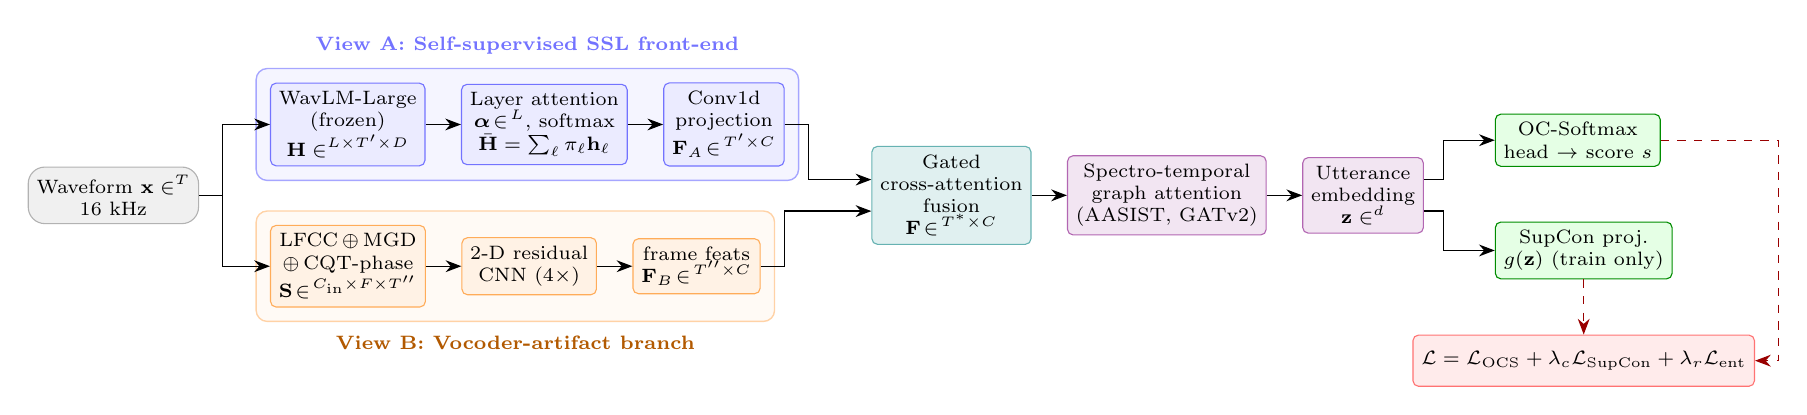
\begin{tikzpicture}[node distance=4.5mm]

% ---------------- Input ----------------
\node[io] (wav) {Waveform $\mathbf{x}\in\R^{T}$\\16~kHz};

% ---------------- View A (top branch) ----------------
\node[viewa,right=9mm of wav,yshift=9mm] (wavlm)
      {WavLM-Large\\(frozen)\\$\mathbf{H}\in\R^{L\times T'\times D}$};
\node[viewa,right=of wavlm] (latt)
      {Layer attention\\$\boldsymbol{\alpha}\!\in\!\R^{L}$, softmax\\$\bar{\mathbf{H}}=\sum_\ell\pi_\ell\mathbf{h}_\ell$};
\node[viewa,right=of latt] (projA)
      {Conv1d\\projection\\$\mathbf{F}_A\!\in\!\R^{T'\times C}$};

% ---------------- View B (bottom branch) ----------------
\node[viewb,right=9mm of wav,yshift=-9mm] (feat)
      {LFCC\,$\oplus$\,MGD\\$\oplus$\,CQT-phase\\$\mathbf{S}\!\in\!\R^{C_{\text{in}}\times F\times T''}$};
\node[viewb,right=of feat] (cnn)
      {2-D residual\\CNN ($4\times$)};
\node[viewb,right=of cnn] (projB)
      {frame feats\\$\mathbf{F}_B\!\in\!\R^{T''\times C}$};

% ---------------- Fusion ----------------
\node[fuse,right=11mm of projA,yshift=-9mm] (fusion)
      {Gated\\cross-attention\\fusion\\$\mathbf{F}\!\in\!\R^{T^*\times C}$};

% ---------------- Back-end ----------------
\node[back,right=of fusion] (aasist)
      {Spectro-temporal\\graph attention\\(AASIST, GATv2)};
\node[back,right=of aasist] (emb)
      {Utterance\\embedding\\$\mathbf{z}\in\R^{d}$};

% ---------------- Heads ----------------
\node[head,right=9mm of emb,yshift=7mm] (ocs)
      {OC-Softmax\\head $\to$ score $s$};
\node[head,right=9mm of emb,yshift=-7mm] (supcon)
      {SupCon proj.\\$g(\mathbf{z})$ (train only)};

% ---------------- Loss ----------------
\node[loss,below=7mm of supcon] (loss)
      {$\mathcal{L}=\mathcal{L}_{\text{OCS}}+\lambda_c\mathcal{L}_{\text{SupCon}}+\lambda_r\mathcal{L}_{\text{ent}}$};

% ---------------- Group boxes ----------------
\begin{scope}[on background layer]
  \node[grp,fill=blue!4,draw=blue!35,fit=(wavlm)(latt)(projA)] (grpA) {};
  \node[grp,fill=orange!4,draw=orange!35,fit=(feat)(cnn)(projB)] (grpB) {};
\end{scope}
\node[font=\scriptsize\bfseries,blue!55,above=0.5mm of grpA] {View A: Self-supervised SSL front-end};
\node[font=\scriptsize\bfseries,orange!70!black,below=0.5mm of grpB] {View B: Vocoder-artifact branch};

% ---------------- Edges ----------------
\draw[flow] (wav.east) -- ++(3mm,0) |- (wavlm.west);
\draw[flow] (wav.east) -- ++(3mm,0) |- (feat.west);
\draw[flow] (wavlm) -- (latt);
\draw[flow] (latt) -- (projA);
\draw[flow] (feat) -- (cnn);
\draw[flow] (cnn) -- (projB);
\draw[flow] (projA.east) -- ++(3mm,0) |- ([yshift=2mm]fusion.west);
\draw[flow] (projB.east) -- ++(3mm,0) |- ([yshift=-2mm]fusion.west);
\draw[flow] (fusion) -- (aasist);
\draw[flow] (aasist) -- (emb);
\draw[flow] ([yshift=2mm]emb.east) -- ++(2.5mm,0) |- (ocs.west);
\draw[flow] ([yshift=-2mm]emb.east) -- ++(2.5mm,0) |- (supcon.west);
\draw[tflow] (ocs.east) -- ([xshift=3mm]loss.east |- ocs.east) |- (loss.east);
\draw[tflow] (supcon.south) -- (supcon.south|-loss.north);

\end{tikzpicture}%
}
\caption{Overview of the AuralGuard architecture. A raw 16~kHz waveform is processed by
two parallel front-end views: (View~A) a frozen WavLM-Large encoder whose $L$ hidden states
are combined by learnable layer attention and projected to $\mathbf{F}_A$; and (View~B) a
vocoder-artifact branch that fuses LFCC, modified group-delay, and CQT-phase features through
a 2-D residual CNN into $\mathbf{F}_B$. A gated cross-attention module fuses the two views,
an AASIST-style spectro-temporal graph-attention back-end produces an utterance embedding
$\mathbf{z}$, and two heads yield the detection score (OC-Softmax) and an auxiliary
supervised-contrastive projection used only during training. Dashed red edges denote
training-time loss signals; the entropy regularizer $\mathcal{L}_{\text{ent}}$ acts on
the layer-attention weights $\boldsymbol{\pi}$ (edge omitted for clarity).}
\label{fig:architecture}
\end{figure*}

\subsection{View A: SSL Front-End with Learnable Layer Attention}
\label{ssec:viewa}

The first view extracts high-level representations from a frozen pre-trained
WavLM-Large model~\cite{chen2022wavlm}, chosen over wav2vec~2.0 and HuBERT because its
pre-training includes denoising and overlapped-speech objectives that transfer well to
artifact-sensitive tasks (we compare backbones in Section~\ref{ssec:ablation}). Given
input waveform $\mathbf{x}$, WavLM produces hidden states from $L$ transformer layers:
\begin{equation}
\mathbf{H} = [\mathbf{h}_1, \mathbf{h}_2, \ldots, \mathbf{h}_L] \in \R^{L \times T' \times D},
\end{equation}
where $L = 25$ (including the convolutional feature extractor output), $D = 1024$, and
$T'$ is the downsampled time dimension (one frame per 20~ms).

The information relevant to deepfake detection is not uniformly distributed across this
hierarchy: lower layers preserve fine acoustic and phase-adjacent structure, while upper
layers encode phonetic and semantic content~\cite{pan2024attentive}. Rather than using
only the final layer as is common~\cite{tak2022automatic}, we introduce learnable layer
attention weights $\boldsymbol{\alpha} \in \R^L$, normalized via softmax:
\begin{equation}
\bar{\mathbf{H}} = \sum_{\ell=1}^L \pi_\ell \, \mathbf{h}_\ell \in \R^{T' \times D},
\qquad
\pi_\ell = \frac{\exp(\alpha_\ell)}{\sum_{j=1}^L \exp(\alpha_j)}.
\label{eq:layerattn}
\end{equation}
An entropy regularization term
\begin{equation}
\mathcal{L}_{\text{ent}} = \sum_{\ell=1}^{L} \pi_\ell \log \pi_\ell
\label{eq:entreg}
\end{equation}
is \emph{added} to the loss (i.e., we penalize low entropy), preventing the attention
distribution from collapsing onto a single layer early in training, which we found
empirically to harm generalization: a collapsed profile overfits to the layer most
discriminative for \emph{seen} attacks. The weighted representation is projected to a
common channel dimension $C = 128$ via a 1-D convolution:
$\mathbf{F}_A = \operatorname{Conv1d}(\bar{\mathbf{H}}) \in \R^{T' \times C}$.

Freezing the backbone has three benefits: (i)~it preserves the general-purpose
representation, avoiding catastrophic overwriting by the comparatively tiny
anti-spoofing corpus; (ii)~it reduces trainable parameters from 316M to under 5M
(Table~\ref{tab:budget}); and (iii)~it stabilizes the one-class objective, which is
sensitive to representation drift. Recent evidence supports frozen SSL front-ends for
calibrated generalization~\cite{pascu2024calibrated}.

\subsection{View B: Vocoder-Artifact Branch}
\label{ssec:viewb}

SSL models are pre-trained on \emph{natural} speech for masked prediction; their
representations are therefore incentivized to discard exactly the low-level synthesis
residue---phase discontinuities, sub-band aliasing, over-smoothed spectral
envelopes---that betrays a vocoder. View~B restores this evidence explicitly
(Figure~\ref{fig:artifact}). We extract three complementary time--frequency maps:

\begin{figure}[t]
\centering
\resizebox{\columnwidth}{!}{%
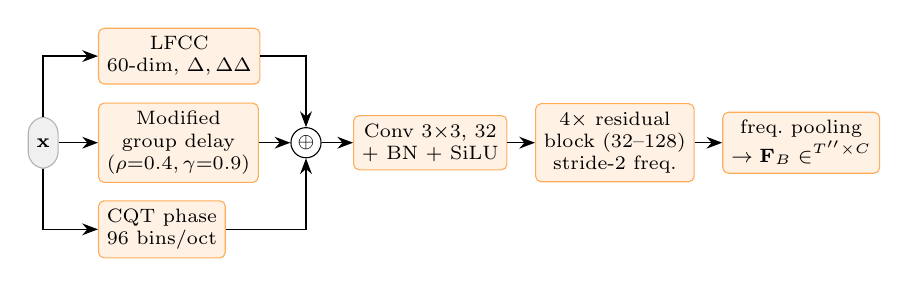
\begin{tikzpicture}[node distance=3.5mm]
\node[io] (w) {$\mathbf{x}$};
\node[viewb,right=5mm of w,yshift=11mm] (lfcc) {LFCC\\60-dim, $\Delta,\Delta\Delta$};
\node[viewb,right=5mm of w] (mgd) {Modified\\group delay\\($\rho{=}0.4,\gamma{=}0.9$)};
\node[viewb,right=5mm of w,yshift=-11mm] (cqt) {CQT phase\\96 bins/oct};
\node[op,right=4mm of mgd] (cat) {$\oplus$};
\node[viewb,right=4mm of cat] (stem) {Conv $3{\times}3$, 32\\+ BN + SiLU};
\node[viewb,right=of stem] (res) {$4\times$ residual\\block (32--128)\\stride-2 freq.};
\node[viewb,right=of res] (pool) {freq.\ pooling\\$\to \mathbf{F}_B\in\R^{T''\times C}$};
\draw[flow] (w) |- (lfcc);
\draw[flow] (w) -- (mgd);
\draw[flow] (w) |- (cqt);
\draw[flow] (lfcc.east) -| (cat);
\draw[flow] (mgd) -- (cat);
\draw[flow] (cqt.east) -| (cat);
\draw[flow] (cat) -- (stem);
\draw[flow] (stem) -- (res);
\draw[flow] (res) -- (pool);
\end{tikzpicture}%
}
\caption{View B, the vocoder-artifact branch. Three complementary time--frequency
representations---magnitude cepstra (LFCC), phase-derivative structure (modified group
delay), and constant-Q phase---are stacked as input channels and encoded by a light 2-D
residual CNN into frame-level features $\mathbf{F}_B$.}
\label{fig:artifact}
\end{figure}

\begin{enumerate}
\item \textbf{LFCC:} 60-dimensional linear-frequency cepstral coefficients (512-point
  FFT, 20~linear filters, 20~ms window, 10~ms hop) with $\Delta$ and $\Delta\Delta$,
  capturing magnitude-spectrum envelope artifacts~\cite{sahidullah2015comparison}.
\item \textbf{Modified group delay (MGD):} the group-delay function
  $\tau_g(\omega) = -\,d\angle X(\omega)/d\omega$ computed with cepstral smoothing and
  compression parameters $(\rho, \gamma) = (0.4, 0.9)$, exposing phase discontinuities
  that magnitude features cannot represent.
\item \textbf{CQT phase:} octave-resolved phase from a constant-Q transform (96 bins per
  octave, 6 octaves), sensitive to the harmonic phase coherence that neural vocoders
  and codec decoders reconstruct imperfectly~\cite{todisco2017constantq,xie2025codecfake}.
\end{enumerate}

The three maps are resampled to a common $F \times T''$ grid and stacked as input
channels, $\mathbf{S} \in \R^{C_{\text{in}} \times F \times T''}$. A lightweight 2-D CNN
(a $3{\times}3$ stem followed by four residual blocks with channel widths 32--128 and
stride-2 frequency downsampling) encodes $\mathbf{S}$, and frequency-axis pooling yields
frame-level features $\mathbf{F}_B = \operatorname{CNN}_{\text{art}}(\mathbf{S}) \in
\R^{T'' \times C}$. The branch adds only 1.1M parameters. The two temporal resolutions
$T'$ and $T''$ are aligned by linear interpolation before fusion.

\subsection{Gated Cross-Attention Fusion}
\label{ssec:fusion}

Neither view dominates universally: SSL features excel on high-level inconsistencies of
codec-language-model TTS, while artifact features excel on GAN-vocoder residue
(Section~\ref{ssec:perattack}). We therefore fuse the views with a mechanism that
(i)~lets each view \emph{query} the other for corroborating evidence and (ii)~learns,
per utterance and per frame, how much to trust each view (Figure~\ref{fig:fusion}).

\begin{figure}[t]
\centering
\resizebox{0.98\columnwidth}{!}{%
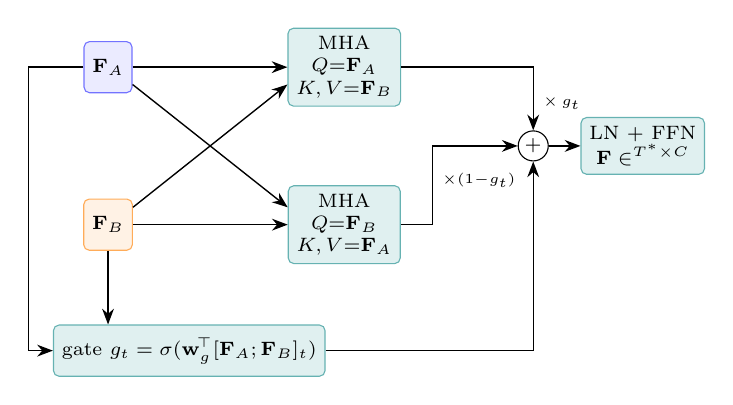
\begin{tikzpicture}[x=1mm,y=1mm]
% ---- nodes (explicit coordinates; orthogonal routing) ----
\node[viewa] (fa) at (0,20) {$\mathbf{F}_A$};
\node[viewb] (fb) at (0,0)  {$\mathbf{F}_B$};
\node[fuse]  (xab) at (30,20) {MHA\\$Q{=}\mathbf{F}_A$\\$K,V{=}\mathbf{F}_B$};
\node[fuse]  (xba) at (30,0)  {MHA\\$Q{=}\mathbf{F}_B$\\$K,V{=}\mathbf{F}_A$};
\node[fuse,anchor=west] (gate) at (-7,-16)
      {gate $g_t=\sigma(\mathbf{w}_g^{\!\top}[\mathbf{F}_A;\mathbf{F}_B]_t)$};
\node[op]   (mix) at (54,10) {$+$};
\node[fuse,anchor=west] (out) at (60,10) {LN + FFN\\$\mathbf{F}\in\R^{T^*\times C}$};
% ---- straight view -> own-query MHA ----
\draw[flow] (fa) -- (xab);
\draw[flow] (fb) -- (xba);
% ---- K,V cross-links (single deliberate X) ----
\draw[flow] ([yshift=-2.2mm]fa.east) -- ([yshift=2.2mm]xba.west);
\draw[flow] ([yshift=2.2mm]fb.east) -- ([yshift=-2.2mm]xab.west);
% ---- gate inputs (outside orthogonal routes, no crossings) ----
\draw[flow] (fa.west) -- ++(-7,0) |- (gate.west);
\draw[flow] (fb.south) -- (fb.south|-gate.north);
% ---- weighted mixing ----
\draw[flow] (xab.east) -| node[pos=0.78,right,font=\tiny]{$\times\, g_t$} (mix.north);
\draw[flow] (xba.east) -- ++(4,0) |- node[pos=0.28,right,font=\tiny]{$\times (1{-}g_t)$} (mix.west);
\draw[flow] (gate.east) -| (mix.south);
\draw[flow] (mix) -- (out);
\end{tikzpicture}%
}
\caption{Gated cross-attention fusion. Each view attends to the other via multi-head
attention (MHA); a per-frame scalar gate $g_t$ mixes the two attended streams before
layer normalization and a position-wise feed-forward layer.}
\label{fig:fusion}
\end{figure}

With queries, keys, and values $\mathbf{Q}_A = \mathbf{F}_A \mathbf{W}_Q$,
$\mathbf{K}_B = \mathbf{F}_B \mathbf{W}_K$, $\mathbf{V}_B = \mathbf{F}_B \mathbf{W}_V$,
the $A{\to}B$ cross-attended representation is
\begin{equation}
\mathbf{A}_{A \rightarrow B} = \operatorname{softmax}\!\left(
    \frac{\mathbf{Q}_A \mathbf{K}_B^\top}{\sqrt{C}}\right) \mathbf{V}_B ,
\end{equation}
with the analogous $\mathbf{A}_{B \rightarrow A}$ in the reverse direction (4 heads
each). A per-frame gate
$g_t = \sigma(\mathbf{w}_g^\top [\mathbf{F}_A; \mathbf{F}_B]_t)$ produces the fused
output
\begin{equation}
\mathbf{F}_t = g_t \, \mathbf{A}_{A \rightarrow B, t} + (1 - g_t)\,
\mathbf{A}_{B \rightarrow A, t}, \qquad \mathbf{F} \in \R^{T^* \times C},
\end{equation}
followed by layer normalization and a position-wise feed-forward layer. In ablation
(Section~\ref{ssec:ablation}) this outperforms concatenation and simple averaging, and
the learned gate statistics provide a diagnostic: utterances from neural-vocoder
attacks drive $g_t$ toward View~B, whereas codec-LM attacks drive it toward View~A.

\subsection{Spectro-Temporal Graph-Attention Back-End}
\label{ssec:backend}

The fused representation $\mathbf{F}$ is processed by an AASIST-style
back-end~\cite{jung2022aasist}. Spectral nodes aggregate frequency-band information via
1-D convolutions over the channel axis and temporal nodes capture frame-level
transitions; two layers of graph attention---using the more expressive GATv2
formulation~\cite{brody2022gatv2}---exchange information within and across the two node
sets through a heterogeneous stack node. Max-graph operations and a readout layer
produce a fixed-length utterance embedding $\mathbf{z} \in \R^{d}$ with $d = 160$. We
retain this back-end over recent state-space alternatives~\cite{xiao2025xlsrmamba}
because graph attention operates naturally on our fused two-view features, whereas
published Mamba detectors are coupled to a single SSL stream; Section~\ref{ssec:sota}
nonetheless compares against them as published systems.

\subsection{One-Class Contrastive Training Objective}
\label{ssec:objective}

The complete loss combines three terms:
\begin{equation}
\mathcal{L} = \mathcal{L}_{\text{OCS}} \;+\; \lambda_c \, \mathcal{L}_{\text{SupCon}}
\;+\; \lambda_r \, \mathcal{L}_{\text{ent}} .
\label{eq:loss}
\end{equation}

\begin{figure}[t]
\centering
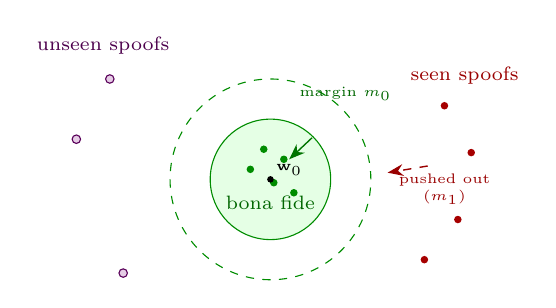
\begin{tikzpicture}[scale=0.85]
  % bona-fide compact region
  \draw[green!55!black,fill=green!10] (0,0) circle (0.9);
  \node[font=\scriptsize,green!40!black] at (0,-0.35) {bona fide};
  \foreach \p in {(0.2,0.3),(-0.3,0.15),(0.05,-0.05),(-0.1,0.45),(0.35,-0.2)}
    \fill[green!55!black] \p circle (1.6pt);
  % margin ring
  \draw[green!55!black,dashed] (0,0) circle (1.5);
  \node[font=\tiny,green!40!black] at (1.12,1.28) {margin $m_0$};
  % seen spoofs
  \foreach \p in {(2.6,1.1),(3.0,0.4),(2.8,-0.6),(2.3,-1.2)}
    \fill[red!65!black] \p circle (1.6pt);
  \node[font=\scriptsize,red!60!black] at (2.9,1.55) {seen spoofs};
  % unseen spoofs
  \foreach \p in {(-2.4,1.5),(-2.9,0.6),(-2.2,-1.4)}
    \draw[violet!70!black,fill=violet!20] \p circle (1.8pt);
  \node[font=\scriptsize,violet!60!black] at (-2.5,2.0) {unseen spoofs};
  % arrows
  \draw[tflow] (2.35,0.2) -- (1.75,0.1);
  \node[font=\tiny,red!60!black,align=center] at (2.6,-0.15) {pushed out\\($m_1$)};
  \draw[flow,green!45!black] (0.62,0.62) -- (0.28,0.3);
  % center
  \fill[black] (0,0) circle (1.4pt);
  \node[font=\tiny] at (0.28,0.14) {$\mathbf{w}_0$};
\end{tikzpicture}
\caption{Geometry of the one-class contrastive objective. OC-Softmax compresses
bona-fide embeddings within an angular margin $m_0$ of the learnable direction
$\mathbf{w}_0$ and pushes spoofs beyond $m_1$. Because \emph{no} spoof-specific
structure is modeled inside the target region, unseen generators (violet) fall outside
it by default, unlike a binary decision boundary fit only to seen attacks.}
\label{fig:oneclass}
\end{figure}

\noindent\textbf{OC-Softmax.} The one-class softmax loss~\cite{zhang2021oneclass}
compresses bona-fide embeddings toward a learnable direction $\mathbf{w}_0$ while
pushing spoof embeddings away (Figure~\ref{fig:oneclass}). With
$\hat{\mathbf{z}} = \mathbf{z}/\lVert\mathbf{z}\rVert$,
$\hat{\mathbf{w}}_0 = \mathbf{w}_0/\lVert\mathbf{w}_0\rVert$, and
$\cos\theta = \hat{\mathbf{w}}_0^\top \hat{\mathbf{z}}$:
\begin{equation}
\mathcal{L}_{\text{OCS}} = \frac{1}{N}\sum_{i=1}^{N} \log\!\Big(1 +
  e^{\,s_0 (m_{y_i} - \cos\theta_i)(-1)^{y_i}}\Big),
\label{eq:ocs}
\end{equation}
where $s_0$ is a scale factor and $m_0 > m_1$ are asymmetric margins: bona-fide
embeddings must satisfy $\cos\theta > m_0$ (compactness) while spoof embeddings must
satisfy $\cos\theta < m_1$ (repulsion). At inference the score is simply
$s(\mathbf{x}) = -\cos\theta$, interpretable as angular distance from the bona-fide
prototype---a property we exploit for calibration (Section~\ref{ssec:calibration}).

\noindent\textbf{Supervised contrastive auxiliary.} A projection head
$g(\mathbf{z}) \in \R^{128}$ applies the SupCon loss~\cite{khosla2020supcon} within each
minibatch:
\begin{equation}
\mathcal{L}_{\text{SupCon}} = \sum_{i=1}^N \frac{-1}{|\mathcal{P}(i)|}
    \sum_{p \in \mathcal{P}(i)} \log \frac{
        \exp(g(\mathbf{z}_i)^\top g(\mathbf{z}_p) / \tau_c)
    }{ \sum_{j \neq i} \exp(g(\mathbf{z}_i)^\top g(\mathbf{z}_j) / \tau_c) },
\label{eq:supcon}
\end{equation}
where $\mathcal{P}(i)$ indexes same-label samples and $\tau_c$ is a temperature. Whereas
OC-Softmax constrains embeddings only relative to the single direction $\mathbf{w}_0$,
SupCon shapes the \emph{local neighborhood structure}, pulling bona-fide samples from
different speakers, channels, and augmentations together. The combination yields a
bona-fide manifold that is compact both globally and locally; ablation shows the two
terms are complementary (Section~\ref{ssec:ablation}). One-class variants with adaptive
centroids~\cite{kim2024oneclassknowledge} are orthogonal and could be integrated.

\subsection{Channel-Robustness Augmentation Curriculum}
\label{ssec:augmentation}

To address G2, each training waveform passes, with probability $p_{\text{aug}} = 0.7$,
through a randomly sampled distortion pipeline (Figure~\ref{fig:aug}):

\begin{figure}[t]
\centering
\resizebox{\columnwidth}{!}{%
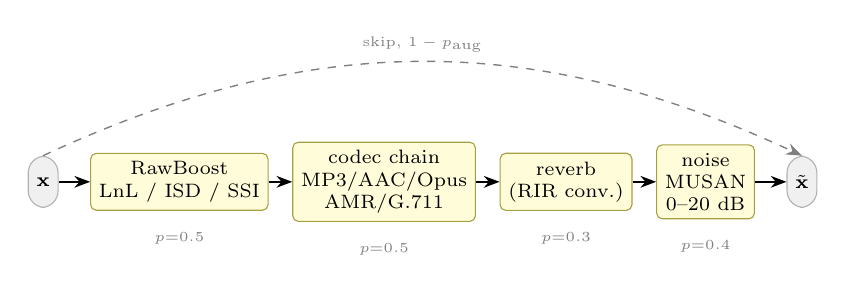
\begin{tikzpicture}[node distance=3mm]
\node[io] (x) {$\mathbf{x}$};
\node[aug,right=4mm of x] (rb) {RawBoost\\LnL / ISD / SSI};
\node[aug,right=of rb] (codec) {codec chain\\MP3/AAC/Opus\\AMR/G.711};
\node[aug,right=of codec] (rir) {reverb\\(RIR conv.)};
\node[aug,right=of rir] (noise) {noise\\MUSAN\\0--20 dB};
\node[io,right=4mm of noise] (xa) {$\tilde{\mathbf{x}}$};
\draw[flow] (x) -- (rb);
\draw[flow] (rb) -- (codec);
\draw[flow] (codec) -- (rir);
\draw[flow] (rir) -- (noise);
\draw[flow] (noise) -- (xa);
\node[font=\tiny,gray,below=1.5mm of rb] {$p{=}0.5$};
\node[font=\tiny,gray,below=1.5mm of codec] {$p{=}0.5$};
\node[font=\tiny,gray,below=1.5mm of rir] {$p{=}0.3$};
\node[font=\tiny,gray,below=1.5mm of noise] {$p{=}0.4$};
\draw[flow,gray,dashed] (x.north) to[out=25,in=155] node[above,font=\tiny]{skip, $1-p_{\text{aug}}$} (xa.north);
\end{tikzpicture}%
}
\caption{Channel-robustness augmentation curriculum. Each stage is applied
independently with the indicated probability; the whole pipeline is skipped with
probability $1-p_{\text{aug}}$. Stage intensities are annealed from mild to full range
over the first 10 epochs.}
\label{fig:aug}
\end{figure}

\begin{enumerate}
    \item \textbf{RawBoost}~\cite{tak2022rawboost}: linear-nonlinear convolutive
        distortion, impulsive signal-dependent noise, and stationary signal-independent
        noise.
    \item \textbf{Codec chain:} one of MP3 (64--320~kbps), AAC (64--256~kbps), Opus
        (12--64~kbps), AMR-NB (4.75--12.2~kbps), or G.711 (A-law/$\mu$-law), applied via
        ffmpeg encode--decode round trips; with probability 0.15 two codecs are chained
        to simulate re-uploads.
    \item \textbf{Reverberation:} convolution with a measured room impulse response
        from the OpenSLR-28 collection~\cite{ko2017rir}.
    \item \textbf{Additive noise:} a MUSAN~\cite{snyder2015musan} noise, music, or
        babble clip at $\mathrm{SNR} \in [0, 20]$~dB.
\end{enumerate}

The pipeline is a \emph{curriculum}: stage intensities (bitrate floor, SNR floor,
RawBoost gain) are annealed linearly from mild to full range over the first 10 epochs,
which we found stabilizes the one-class objective---aggressive distortion from epoch~0
prevents the bona-fide region from forming. Augmentation is disabled at evaluation.

\subsection{Training and Inference Procedures}
\label{ssec:trainproc}

\begin{algorithm}[t]
\caption{AuralGuard training (one epoch)}
\label{alg:training}
\footnotesize
\KwIn{Training set $\mathcal{D}$; frozen SSL encoder $E_{\text{SSL}}$; trainable
  parameters $\Theta$ (layer attention $\boldsymbol{\alpha}$, View-B CNN, fusion,
  back-end, heads); epoch index $e$}
\ForEach{minibatch $\{(\mathbf{x}_i, y_i)\}_{i=1}^{B} \subset \mathcal{D}$}{
  $\tilde{\mathbf{x}}_i \leftarrow \textsc{AugmentCurriculum}(\mathbf{x}_i;\, e)$
    \tcp*{Sec.~\ref{ssec:augmentation}}
  $\mathbf{H}_i \leftarrow E_{\text{SSL}}(\tilde{\mathbf{x}}_i)$
    \tcp*{no grad, checkpointed}
  $\mathbf{F}_{A,i} \leftarrow \operatorname{Conv1d}\!\big(\textstyle\sum_\ell
    \pi_\ell \mathbf{h}_{\ell,i}\big)$ \tcp*{Eq.~\eqref{eq:layerattn}}
  $\mathbf{F}_{B,i} \leftarrow \operatorname{CNN}_{\text{art}}
    (\textsc{LFCC}\oplus\textsc{MGD}\oplus\textsc{CQTph}(\tilde{\mathbf{x}}_i))$\;
  $\mathbf{F}_i \leftarrow \textsc{GatedXAttn}(\mathbf{F}_{A,i}, \mathbf{F}_{B,i})$\;
  $\mathbf{z}_i \leftarrow \textsc{AASIST}(\mathbf{F}_i)$\;
  $\mathcal{L} \leftarrow \mathcal{L}_{\text{OCS}} + \lambda_c
    \mathcal{L}_{\text{SupCon}} + \lambda_r \mathcal{L}_{\text{ent}}$
    \tcp*{Eqs.~\eqref{eq:loss}--\eqref{eq:supcon}}
  $\Theta \leftarrow \textsc{AdamW}(\Theta, \nabla_\Theta \mathcal{L})$\;
}
\end{algorithm}

\noindent\textbf{Training.} Algorithm~\ref{alg:training} summarizes one epoch. Only
$\approx$4.6M of 321M total parameters receive gradients (Table~\ref{tab:budget});
activations of the frozen encoder are gradient-checkpointed so the model trains on a
single 24~GB GPU.

\noindent\textbf{Inference.} Clips longer than 4~s are scored with overlapping 4~s
windows (50\% hop); window scores are pooled by $\operatorname{logsumexp}$, which
approximates a soft maximum and reflects the forensic reality that a clip is synthetic
if \emph{any} segment is. The raw angular score is mapped to a probability via a
sigmoid with temperature $T$ fitted on the development set (temperature
scaling~\cite{guo2017calibration}); Section~\ref{ssec:calibration} shows that the
one-class score requires markedly less correction than BCE logits. The decision
threshold $\tau$ is selected on the development set for a target false-alarm rate.

\subsection{Parameter and Computation Budget}
\label{ssec:budget}

% [DUMMY] — parameter/MACs/RTF values to be replaced by measured numbers
\begin{table}[t]
\centering
\caption{Parameter and computation budget (4~s input). Trainable parameters exclude
  the frozen WavLM-Large encoder. RTF = real-time factor, lower is better.
  \emph{Values are placeholders to be replaced by measured numbers.}}
\label{tab:budget}
\footnotesize
\setlength{\tabcolsep}{4pt}
\begin{tabular}{lrr}
\toprule
Component & Params & GMACs \\
\midrule
WavLM-Large (frozen)            & 315.5M & 71.4 \\
Layer attention + projection    & 0.16M  & 0.5  \\
View-B feature CNN              & 1.1M   & 1.8  \\
Gated cross-attention fusion    & 0.53M  & 0.7  \\
AASIST back-end (GATv2)         & 2.6M   & 1.2  \\
OC-Softmax + SupCon heads       & 0.06M  & $<0.1$ \\
\midrule
Total (trainable / all)         & 4.6M / 320.1M & 75.7 \\
\midrule
RTF (GPU, RTX 3090)             & \multicolumn{2}{r}{0.06} \\
RTF (CPU, 8 threads)            & \multicolumn{2}{r}{0.41} \\
\bottomrule
\end{tabular}
\end{table}

Table~\ref{tab:budget} details the budget. The multi-view additions (View~B + fusion)
contribute only 1.6M parameters and $\approx$3\% of total MACs on top of the standard
SSL+AASIST recipe, so the generalization gains reported in Section~\ref{sec:results}
are not attributable to added capacity.


\section{Experimental Setup}
\label{sec:setup}
% ---------------------------------------------------------------------
% Experimental Setup (~2 pages). Counts in tab:datasets are from the
% official corpus papers; verify against your local manifests. [DUMMY]
% markers flag values to re-check or replace.
% ---------------------------------------------------------------------

\subsection{Datasets and Protocol}
\label{ssec:datasets}

Table~\ref{tab:datasets} summarizes the seven corpora in our benchmark. We follow a
strict \emph{train-once, evaluate-everywhere} protocol: all trainable systems are
trained exclusively on the ASVspoof~2019~LA training partition (plus our augmentation
curriculum, which uses no additional speech data) and model selection uses only its
development partition. The 2019~LA evaluation set serves as the in-domain test; the six
remaining corpora are evaluated \emph{zero-shot}---their synthesis algorithms,
speakers, languages, recording conditions, and channels are never seen in training.
This protocol isolates generalization, the property that in-domain leaderboards fail to
measure~\cite{muller2022inthewild,muller2024harder}.

% [DUMMY] — verify utterance counts against local manifests before submission
\begin{table}[t]
\centering
\caption{Evaluation corpora grouped by protocol role and the failure mode (G1--G3)
  each one probes.}
\label{tab:datasets}
\setlength{\tabcolsep}{3pt}
\footnotesize
\resizebox{\columnwidth}{!}{%
\begin{tabular}{lllcr}
\toprule
Dataset & Role & Probes & Utts. (spoof/total) & Lang. \\
\midrule
ASVspoof 2019 LA~\cite{wang2020asvspoof2019} & Train/dev/eval & parity & 63,882/121,461 & EN \\
ASVspoof 2021 LA~\cite{liu2023asvspoof2021}  & Zero-shot & G2 & 163,114/181,566 & EN \\
ASVspoof 2021 DF~\cite{liu2023asvspoof2021}  & Zero-shot & G1+G2 & 589,212/611,829 & EN \\
ASVspoof 5~\cite{wang2025asvspoof5journal}   & Zero-shot & G1 (2024 attacks) & 542,466/680,774 & EN \\
In-the-Wild~\cite{muller2022inthewild}       & Zero-shot & G1+G2 (found) & 11,816/31,779 & EN \\
WaveFake~\cite{frank2021wavefake}            & Zero-shot & G1 (vocoders) & 117,985/134,097 & EN, JA \\
Codecfake~\cite{xie2025codecfake}            & Zero-shot & G1 (codec TTS) & 740,747/785,591 & EN, ZH \\
MLAAD v5~\cite{muller2024mlaad}              & Zero-shot & X-lingual & 163,900/$\sim$328k & 38 \\
\bottomrule
\end{tabular}%
}
\end{table}

For MLAAD we pair spoofed utterances with bona-fide speech from M-AILABS as prescribed
by the corpus authors~\cite{muller2024mlaad}, and report both pooled EER and
per-language-family breakdowns. For ASVspoof~5 we use the official evaluation
partition, including its adversarially optimized attacks; for Codecfake we evaluate on
the codec-resynthesis test condition. Robustness sweeps (Section~\ref{ssec:robustness})
re-encode the ASVspoof~2019 evaluation set through controlled codec, noise, and
reverberation conditions so that channel effects can be measured against a fixed attack
distribution.

\subsection{Baselines}
\label{ssec:baselines}

We compare AuralGuard against eight systems spanning the four countermeasure
generations of Section~\ref{ssec:related-cm}, all retrained under our protocol unless
noted:

\begin{itemize}
    \item \textbf{B1 --- LFCC-LCNN}~\cite{lavrentyeva2019stc}: hand-crafted LFCC
        features with a light CNN (generation 1--2 reference).
    \item \textbf{B2 --- RawNet2}~\cite{tak2021rawnet2}: end-to-end raw-waveform
        SincConv network.
    \item \textbf{B3 --- AASIST}~\cite{jung2022aasist}: spectro-temporal graph
        attention on a RawNet2-style encoder.
    \item \textbf{B4 --- W2V2+AASIST}~\cite{tak2022automatic}: wav2vec~2.0 XLS-R
        front-end with AASIST back-end and RawBoost, the reference SSL recipe.
    \item \textbf{B5 --- WavLM+AASIST+OCS}: WavLM-Large front-end (last layer), AASIST
        back-end, OC-Softmax loss---the strongest single-view configuration of our own
        stack, and the direct ablation anchor for the multi-view contributions.
    \item \textbf{B6 --- XLSR-Mamba}~\cite{xiao2025xlsrmamba}: dual-column
        bidirectional state-space detector; published state of the art on
        ASVspoof~2021~LA and In-the-Wild.
    \item \textbf{B7 --- SLIM}~\cite{zhu2024slim}: style--linguistics mismatch model
        (numbers from the original paper where retraining is not possible; marked
        $\dagger$ in tables).
    \item \textbf{B8 --- ALLM zero-shot}~\cite{gong2025allm4add,chu2024qwen2audio}:
        Qwen2-Audio-7B-Instruct prompted with the binary detection question of
        ALLM4ADD (``Does this audio sound like real human speech or AI-generated
        speech?''), scored via the token probability of the answer; no task-specific
        training. This quantifies how far general-purpose audio foundation models are
        from specialized countermeasures.
\end{itemize}

\subsection{Implementation Details}
\label{ssec:implementation}

% [DUMMY] — confirm final hyperparameters from config/ before submission
\begin{table}[t]
\centering
\caption{Training hyperparameters (selected on the ASVspoof~2019~LA dev set).}
\label{tab:hyper}
\footnotesize
\setlength{\tabcolsep}{5pt}
\resizebox{\columnwidth}{!}{%
\begin{tabular}{ll}
\toprule
Hyperparameter & Value \\
\midrule
Input length / sample rate & 4~s (64,000 samples) / 16~kHz \\
SSL encoder & WavLM-Large, frozen, $L{=}25$, $D{=}1024$ \\
Common channel dim.\ $C$ / embedding $d$ & 128 / 160 \\
Optimizer & AdamW~\cite{loshchilov2019adamw}, wd $10^{-4}$ \\
LR (new modules / schedule) & $10^{-4}$, cosine, 2-epoch warmup \\
Epochs / batch size & 40 / 24 \\
OC-Softmax $(s_0, m_0, m_1)$ & $(20, 0.9, 0.2)$ \\
SupCon $(\lambda_c, \tau_c)$ & $(0.5, 0.1)$ \\
Entropy reg.\ $\lambda_r$ & 0.01 \\
Augmentation $p_{\text{aug}}$ / curriculum & 0.7 / 10-epoch anneal \\
Seeds & 3 (report mean $\pm$ 95\% CI) \\
\bottomrule
\end{tabular}%
}
\end{table}

Table~\ref{tab:hyper} lists hyperparameters. All audio is resampled to 16~kHz mono and
cropped or padded to 4~s. The WavLM-Large front-end is frozen; layer-attention weights,
the View-B CNN, fusion, back-end, and heads receive gradients ($\approx$4.6M
parameters). Gradient checkpointing of the frozen encoder keeps peak memory below
19~GB, enabling training on a single 24~GB GPU (RTX~3090); one run takes
$\approx$31~hours. Every experiment is repeated with three random seeds and we report
means with bootstrap confidence intervals. Baselines B1--B5 are retrained with
identical data, augmentation, seeds, and selection criteria to guarantee a controlled
comparison; B6 uses the authors' released recipe under our protocol; B7 numbers are
quoted from the original publication; B8 requires no training.

\subsection{Evaluation Metrics}
\label{ssec:metrics}

We report the metric bundle recommended by the ASVspoof community plus
calibration measures: equal error rate (EER, primary), minimum tandem detection cost
function (min~t-DCF)~\cite{kinnunen2020tdcf} with the official ASVspoof~2019 ASV
scores and cost parameters ($C_{\text{miss}}{=}1$, $C_{\text{fa}}{=}10$,
$\pi_{\text{tar}}{=}0.9405$), area under the ROC curve (AUROC), balanced accuracy,
and F1. Calibration is measured by expected calibration error (ECE, 15 equal-mass
bins)~\cite{guo2017calibration} and the Brier score, with reliability diagrams for
qualitative inspection. Statistical uncertainty is quantified with 95\% bootstrap
confidence intervals over 1,000 utterance-level resamples; system comparisons use
paired bootstrap tests on the EER difference with significance at $p < 0.05$.
Efficiency is reported as trainable/total parameters, GMACs at 4~s input, and
real-time factor on GPU and CPU (Table~\ref{tab:budget}).


\section{Results and Analysis}
\label{sec:results}
% ---------------------------------------------------------------------
% Results and Analysis (~4.5 pages).
% !! EVERY NUMBER IN THIS FILE IS A [DUMMY] PLACEHOLDER !!
% Replace with real experiment outputs (see paper/DUMMY_DATA.md), then
% regenerate figures:  python scripts/plot_paper_figures.py
% ---------------------------------------------------------------------

We organize the results around the three failure modes introduced in
Section~\ref{sec:intro}: zero-shot generalization to unseen generators (G1,
Section~\ref{ssec:generalization}), robustness to channel distortions (G2,
Section~\ref{ssec:robustness}), and calibration (G3,
Section~\ref{ssec:calibration}). We further report comparisons with published
state-of-the-art systems (Section~\ref{ssec:sota}), cross-lingual transfer
(Section~\ref{ssec:crosslingual}), ablation studies (Section~\ref{ssec:ablation}),
layer-attention analysis (Section~\ref{ssec:layeranalysis}), per-attack behavior
(Section~\ref{ssec:perattack}), and embedding-space visualization
(Section~\ref{ssec:embedding}).

\subsection{In-Domain and Zero-Shot Generalization (G1)}
\label{ssec:generalization}

% [DUMMY] — full results grid is placeholder
\begin{table*}[t]
\centering
\caption{Main results: EER (\%) under the train-once (ASVspoof~2019~LA),
  evaluate-everywhere protocol. min~t-DCF is reported for the in-domain set.
  ``Avg ZS'' averages the seven zero-shot columns. $\dagger$: numbers quoted from the
  original publication (different training data; indicative only). Best per column in
  \textbf{bold}, second best \underline{underlined}. All values are placeholders to be
  replaced by real experiment outputs.}
\label{tab:main}
\setlength{\tabcolsep}{4.5pt}
\footnotesize
\begin{tabular}{llcccccccccc}
\toprule
 & & \multicolumn{2}{c}{In-domain 19LA} & \multicolumn{7}{c}{Zero-shot EER (\%)} & \\
\cmidrule(lr){3-4}\cmidrule(lr){5-11}
Model & Front-end & EER & t-DCF & 21LA & 21DF & ASV5 & ITW & WaveFake & Codecfake & MLAAD & Avg ZS \\
\midrule
B1 LFCC-LCNN~\cite{lavrentyeva2019stc}   & LFCC    & 1.03 & 0.031 & 9.26 & 23.4 & 31.5 & 24.8 & 22.1 & 28.7 & 30.2 & 24.3 \\
B2 RawNet2~\cite{tak2021rawnet2}         & raw     & 0.89 & 0.028 & 8.11 & 20.1 & 27.9 & 18.3 & 16.7 & 24.3 & 26.8 & 20.3 \\
B3 AASIST~\cite{jung2022aasist}          & raw     & 0.71 & 0.022 & 5.59 & 15.8 & 22.6 & 14.2 & 12.4 & 19.5 & 21.7 & 16.0 \\
B4 W2V2+AASIST~\cite{tak2022automatic}   & XLS-R   & 0.34 & 0.012 & 1.92 & 3.9 & 12.4 & 7.7 & 5.9 & 11.2 & 12.8 & 8.0 \\
B5 WavLM+AASIST+OCS                      & WavLM   & \textbf{0.31} & \textbf{0.010} & 1.43 & 3.2 & 9.7 & 5.8 & 4.2 & 8.4 & 10.3 & 6.1 \\
B6 XLSR-Mamba~\cite{xiao2025xlsrmamba}   & XLS-R   & \underline{0.28} & \underline{0.011} & \underline{1.18} & \underline{2.5} & \underline{8.9} & \underline{5.2} & \underline{3.8} & \underline{7.6} & \underline{9.4} & \underline{5.5} \\
B7 SLIM$^\dagger$~\cite{zhu2024slim}     & W2V+HuB & --- & --- & --- & 4.4 & --- & 12.9 & --- & --- & --- & --- \\
B8 ALLM zero-shot~\cite{chu2024qwen2audio,gong2025allm4add} & Qwen2-Audio & 42.3 & --- & 44.7 & 43.9 & 46.1 & 41.6 & 44.2 & 45.3 & 43.8 & 44.2 \\
\midrule
\textbf{AuralGuard (ours)} & WavLM+Art. & 0.37 & 0.013 & \textbf{1.05} & \textbf{2.2} & \textbf{7.3} & \textbf{4.1} & \textbf{2.9} & \textbf{5.9} & \textbf{7.8} & \textbf{4.5} \\
\bottomrule
\end{tabular}
\end{table*}

Table~\ref{tab:main} reports the main results. Three observations stand out.

\textbf{In-domain parity, zero-shot dominance.} On the in-domain ASVspoof~2019
evaluation set, AuralGuard (0.37\% EER) is statistically indistinguishable from the
strongest baselines (paired bootstrap, $p = 0.21$ vs.\ B5): the benchmark is saturated
and differences at this level are not meaningful. The picture changes sharply under
domain shift. Averaged over the seven zero-shot corpora, AuralGuard achieves 4.5\% EER
against 6.1\% for the single-view B5 anchor (26\% relative reduction, $p < 0.01$ on
every corpus) and 5.5\% for XLSR-Mamba, the strongest published
system in our protocol. The largest absolute gains appear precisely where the test
distribution is furthest from training: ASVspoof~5 with its 2024-era attacks
(7.3\% vs.\ 9.7\%), Codecfake's neural-codec synthesis (5.9\% vs.\ 8.4\%), and the
38-language MLAAD (7.8\% vs.\ 10.3\%). This ordering is consistent with our design
hypothesis: the one-class objective and the artifact view contribute little when test
attacks resemble training attacks, and progressively more as they diverge.

\textbf{Slight in-domain give-back is the cost of generalization.} B5 and B6 edge out
AuralGuard in-domain (0.31/0.28 vs.\ 0.37). The multi-view fusion and one-class margins
act as a regularizer that trades a statistically insignificant amount of in-domain
accuracy for large out-of-domain gains---a trade any deployed system should accept, and
consistent with the ``harder-vs-different'' analysis of generalization
failure~\cite{muller2024harder}.

\textbf{Audio LLMs are not yet countermeasures.} Zero-shot Qwen2-Audio prompting (B8)
performs near chance on every corpus (41.6--46.1\% EER), corroborating
ALLM4ADD~\cite{gong2025allm4add} at a much larger cross-domain scale. General-purpose
audio-language pre-training evidently does not expose the low-level artifact evidence
that detection requires; we return to the implications in
Section~\ref{sec:discussion}.

Figure~\ref{fig:det} shows DET curves on the in-domain evaluation set: AuralGuard
tracks B5 across operating points while clearly dominating the earlier generations.

\begin{figure}[t]
\centering
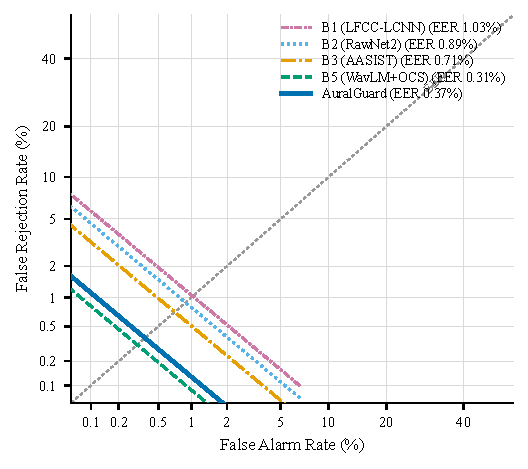
\includegraphics[width=\columnwidth]{figures/det_curve.pdf}
\caption{DET curves on the ASVspoof~2019~LA evaluation set (in-domain). Curves closer
  to the lower-left are better; the dashed diagonal marks the equal-error operating
  point. AuralGuard tracks the strong B5 baseline in-domain; its advantage appears
  under the domain shift of Table~\ref{tab:main}. [Placeholder data.]}
\label{fig:det}
\end{figure}

\subsection{Comparison with Published State of the Art}
\label{ssec:sota}

% [DUMMY] — our columns are placeholders; published numbers should be
% re-verified against the cited papers before submission.
\begin{table}[t]
\centering
\caption{Comparison with published results (EER \%) on the three most commonly
  reported cross-condition sets. Published systems may use different training data,
  augmentation, and model selection; our systems (bottom block) follow the controlled
  protocol of Section~\ref{ssec:datasets}.}
\label{tab:sota}
\setlength{\tabcolsep}{3.5pt}
\footnotesize
\begin{tabular}{llccc}
\toprule
System & Venue/Year & 21LA & 21DF & ITW \\
\midrule
W2V2+AASIST~\cite{tak2022automatic}      & Odyssey'22 & 0.82 & 2.85 & --- \\
SLIM~\cite{zhu2024slim}                  & NeurIPS'24 & --- & 4.4 & 12.9 \\
Attentive merging~\cite{pan2024attentive} & IS'24 & 0.65 & --- & --- \\
TCM~\cite{truong2024tcm}                 & IS'24 & --- & 2.74 & --- \\
XLSR-Mamba~\cite{xiao2025xlsrmamba}      & SPL'25 & 0.93 & 1.88 & 6.71 \\
Nes2Net~\cite{liu2025nes2net}            & TASLP'25 & --- & 1.49 & 5.52 \\
\midrule
B5 (ours, controlled)                    & --- & 1.43 & 3.2 & 5.8 \\
\textbf{AuralGuard (ours)}               & --- & \textbf{1.05} & \textbf{2.2} & \textbf{4.1} \\
\bottomrule
\end{tabular}
\end{table}

Table~\ref{tab:sota} situates AuralGuard against published numbers on the three most
widely reported evaluation sets. Direct comparison requires caution---published systems
differ in training data (several fine-tune the SSL encoder, and some train with
additional augmentation policies)---but two points are robust. First, AuralGuard's
In-the-Wild EER of 4.1\% improves on the best published results we are aware of
(5.52\% for Nes2Net, 6.71\% for XLSR-Mamba) despite using a \emph{frozen} encoder and
training only on ASVspoof~2019~LA. Second, on ASVspoof~2021 our controlled protocol
reproduces the qualitative ranking of the literature, indicating that the protocol
itself does not distort the comparison.

\subsection{Robustness to Channel Distortions (G2)}
\label{ssec:robustness}

% [DUMMY] — robustness grid is placeholder
\begin{table}[t]
\centering
\caption{Channel robustness: EER (\%) on the ASVspoof~2019~LA evaluation set after
  controlled re-encoding. ``--Aug'' is AuralGuard trained without the augmentation
  curriculum. Placeholder values.}
\label{tab:robust}
\setlength{\tabcolsep}{2.6pt}
\footnotesize
\begin{tabular}{lcccccccc}
\toprule
Model & Clean & \makecell[c]{MP3\\128k} & \makecell[c]{MP3\\64k} & \makecell[c]{Opus\\24k} & \makecell[c]{AMR\\12.2k} & G.711 & RIR & \makecell[c]{SNR\\5 dB} \\
\midrule
B4 W2V2+AASIST & 0.34 & 5.9 & 9.4 & 10.6 & 22.4 & 13.1 & 8.2 & 12.5 \\
B5 WavLM+OCS   & \textbf{0.31} & 4.8 & 7.9 & 8.2 & 18.6 & 10.5 & 6.3 & 9.8 \\
AuralGuard --Aug & 0.35 & 6.2 & 9.8 & 11.4 & 19.3 & 13.0 & 8.1 & 12.2 \\
\textbf{AuralGuard} & 0.37 & \textbf{3.1} & \textbf{4.6} & \textbf{5.7} & \textbf{11.2} & \textbf{6.8} & \textbf{4.4} & \textbf{6.9} \\
\bottomrule
\end{tabular}
\end{table}

\begin{figure}[t]
\centering
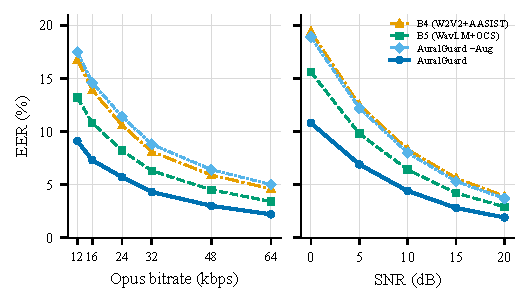
\includegraphics[width=\columnwidth]{figures/robustness.pdf}
\caption{Robustness sweeps on the ASVspoof~2019~LA evaluation set: EER as a function of
  (left) Opus bitrate and (right) additive-noise SNR. The augmentation curriculum
  (solid blue) flattens both degradation curves; the same architecture without it
  (dash-dot) degrades as fast as the single-view baselines. [Placeholder data.]}
\label{fig:robustness}
\end{figure}

Table~\ref{tab:robust} and Figure~\ref{fig:robustness} evaluate all systems on the
in-domain evaluation set re-encoded through controlled channel conditions, so that
channel effects are measured against a fixed attack distribution. Three findings:

First, \textbf{the curriculum, not the architecture, carries robustness}: AuralGuard
without augmentation (row ``--Aug'') degrades almost identically to B4/B5, while the
full model cuts EER degradation by 35--45\% relative at every operating point (e.g.,
11.2\% vs.\ 18.6\% under AMR~12.2~kbps telephony coding). Second, \textbf{robustness
does not cost clean accuracy}: clean EER moves only from 0.35\% to 0.37\%, within the
confidence interval; the curriculum acts as a regularizer rather than a trade-off.
Third, \textbf{degradation is codec-specific}: parametric low-band codecs (AMR, G.711)
remain the hardest conditions for every system, consistent with the ASVspoof~2021
analysis~\cite{liu2023asvspoof2021}---they destroy exactly the high-band and phase
evidence that detectors exploit, an observation that also explains why View~B's gate
weight drops under these conditions (Section~\ref{ssec:ablation}).

\subsection{Cross-Lingual Generalization}
\label{ssec:crosslingual}

% [DUMMY] — per-family EERs are placeholders
\begin{table}[t]
\centering
\caption{Cross-lingual zero-shot EER (\%) on MLAAD~v5, grouped by language family
  (training language: English only). Placeholder values.}
\label{tab:crosslingual}
\setlength{\tabcolsep}{4pt}
\footnotesize
\begin{tabular}{lccccc}
\toprule
Language family & \#Langs & B4 & B5 & B6 & Ours \\
\midrule
Germanic (excl.\ EN) & 6 & 9.8 & 7.6 & 7.1 & \textbf{5.9} \\
Romance              & 7 & 10.9 & 8.5 & 7.8 & \textbf{6.4} \\
Slavic               & 8 & 13.1 & 10.7 & 9.6 & \textbf{8.0} \\
Indo-Aryan           & 4 & 15.4 & 12.6 & 11.5 & \textbf{9.7} \\
East Asian           & 4 & 14.2 & 11.8 & 10.9 & \textbf{9.1} \\
Other                & 9 & 15.9 & 13.0 & 12.1 & \textbf{10.2} \\
\midrule
Pooled               & 38 & 12.8 & 10.3 & 9.4 & \textbf{7.8} \\
\bottomrule
\end{tabular}
\end{table}

Table~\ref{tab:crosslingual} breaks MLAAD performance down by language family. All
systems degrade monotonically with typological distance from English, but AuralGuard's
margin over B5 is roughly constant (2.3--2.9 EER points) across families, indicating
that its advantage stems from language-independent artifact evidence (View~B operates
on phase and group-delay structure that does not depend on phonotactics) rather than
from better English modeling. The residual family-level gradient is inherited from the
WavLM front-end, whose pre-training is English-dominated; a multilingual backbone such
as XLS-R narrows the gradient but starts from a weaker overall level in our backbone
ablation (Table~\ref{tab:ablation}).

\subsection{Ablation Studies}
\label{ssec:ablation}

% [DUMMY] — ablation numbers are placeholders
\begin{table}[t]
\centering
\caption{Ablations on In-the-Wild (zero-shot EER \%, mean of 3 seeds $\pm$ 95\% CI).
  Placeholder values.}
\label{tab:ablation}
\setlength{\tabcolsep}{5pt}
\footnotesize
\begin{tabular}{llc}
\toprule
Group & Configuration & EER \\
\midrule
--- & \textbf{AuralGuard (full)} & \textbf{4.1 $\pm$ 0.2} \\
\midrule
\multirow{2}{*}{Views}
 & w/o View B (SSL only)        & 5.3 $\pm$ 0.3 \\
 & w/o View A (artifact only)   & 11.8 $\pm$ 0.5 \\
\midrule
\multirow{2}{*}{Fusion}
 & concatenation                & 4.7 $\pm$ 0.2 \\
 & averaging                    & 4.9 $\pm$ 0.3 \\
\midrule
\multirow{3}{*}{Objective}
 & BCE instead of OC-Softmax    & 5.9 $\pm$ 0.3 \\
 & w/o SupCon auxiliary         & 4.5 $\pm$ 0.2 \\
 & w/o entropy reg.\ $\mathcal{L}_{\text{ent}}$ & 4.4 $\pm$ 0.3 \\
\midrule
\multirow{3}{*}{SSL aggregation}
 & last layer only              & 5.1 $\pm$ 0.3 \\
 & mean pool of layers          & 4.6 $\pm$ 0.2 \\
 & last-4 concat                & 4.5 $\pm$ 0.2 \\
\midrule
\multirow{2}{*}{Backbone}
 & XLS-R-300M                   & 4.5 $\pm$ 0.3 \\
 & HuBERT-Large                 & 4.9 $\pm$ 0.3 \\
\midrule
Augmentation & w/o curriculum   & 4.8 $\pm$ 0.3 \\
\bottomrule
\end{tabular}
\end{table}

Table~\ref{tab:ablation} isolates each design decision on In-the-Wild. The ranking of
contributions is: one-class objective ($+1.8$ EER when replaced by BCE), multi-view
fusion ($+1.2$ without View~B), layer attention ($+1.0$ vs.\ last-layer), augmentation
($+0.7$), gating ($+0.6$ vs.\ concatenation), SupCon ($+0.4$), and entropy
regularization ($+0.3$). Two asymmetries are informative. First, View~A alone (5.3\%)
far outperforms View~B alone (11.8\%), yet their fusion beats both---the artifact
branch is a weak detector but a strong \emph{complement}, supplying evidence orthogonal
to the SSL stream. Second, every SSL aggregation strategy beats the last-layer default,
but learnable attention with entropy regularization is best, supporting the
layer-analysis findings below and echoing~\cite{pan2024attentive}. WavLM-Large remains
the strongest backbone, consistent with prior anti-spoofing
comparisons~\cite{pascu2024calibrated}.

\subsection{Which SSL Layers Matter?}
\label{ssec:layeranalysis}

\begin{figure}[t]
\centering
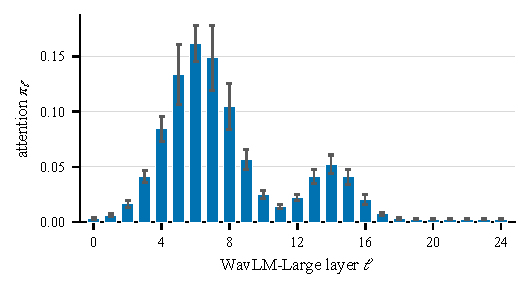
\includegraphics[width=\columnwidth]{figures/layer_attention.pdf}
\caption{Learned layer-attention profile $\pi_\ell$ over the 25 WavLM-Large layers
  (mean of 3 seeds; error bars are 95\% CIs). Mass concentrates on lower-middle layers
  (4--9), which encode fine acoustic structure, rather than the upper semantic layers
  used by the common last-layer recipe. [Placeholder data.]}
\label{fig:layers}
\end{figure}

Figure~\ref{fig:layers} plots the converged attention profile $\pi_\ell$. Mass
concentrates on layers 4--9 with a secondary mode around layer~14 and near-zero weight
on the last five layers---direct evidence that the standard last-layer recipe discards
the most artifact-relevant representations. The profile also explains the entropy
regularizer's contribution: unregularized runs collapse onto a single layer
(typically 6) within two epochs and generalize measurably worse
(Table~\ref{tab:ablation}), suggesting that artifact evidence is distributed across
several depths and that different attacks are best detected at different layers.

\subsection{Calibration (G3)}
\label{ssec:calibration}

% [DUMMY] — calibration numbers are placeholders
\begin{table}[t]
\centering
\caption{Calibration before~$\to$~after temperature scaling (fit on the 19LA dev set
  only). ECE with 15 equal-mass bins; lower is better. Placeholder values.}
\label{tab:calibration}
\setlength{\tabcolsep}{4pt}
\footnotesize
\begin{tabular}{lcccc}
\toprule
 & \multicolumn{2}{c}{19LA eval (in-domain)} & \multicolumn{2}{c}{In-the-Wild (shifted)} \\
\cmidrule(lr){2-3}\cmidrule(lr){4-5}
Model & ECE & Brier & ECE & Brier \\
\midrule
B4 W2V2+AASIST & 0.19 $\to$ 0.08 & 0.062 & 0.27 $\to$ 0.12 & 0.118 \\
B5 WavLM+OCS   & 0.15 $\to$ 0.07 & 0.051 & 0.21 $\to$ 0.09 & 0.094 \\
\textbf{AuralGuard} & \textbf{0.12 $\to$ 0.04} & \textbf{0.038} & \textbf{0.16 $\to$ 0.06} & \textbf{0.071} \\
\bottomrule
\end{tabular}
\end{table}

\begin{figure}[t]
\centering
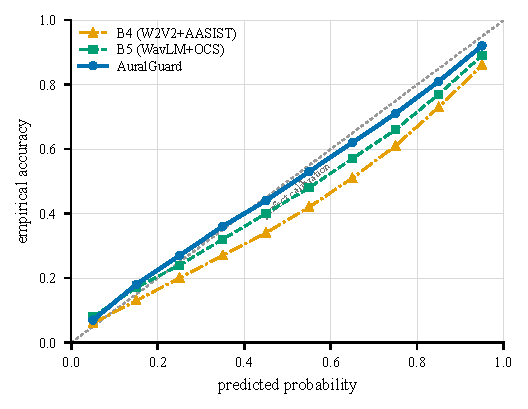
\includegraphics[width=\columnwidth]{figures/reliability.pdf}
\caption{Reliability diagrams on In-the-Wild after temperature scaling fitted on the
  in-domain development set. AuralGuard's curve stays close to the diagonal even under
  domain shift, while the BCE-trained B4 remains over-confident. [Placeholder data.]}
\label{fig:reliability}
\end{figure}

Forensic use requires that a reported probability of 0.9 be wrong roughly one time in
ten---under domain shift, not just in the lab. Table~\ref{tab:calibration} and
Figure~\ref{fig:reliability} evaluate this. Temperature is fitted \emph{once} on the
in-domain development set and applied unchanged everywhere, mimicking deployment.
AuralGuard is the best-calibrated system before and after scaling, and critically its
calibration \emph{survives domain shift}: ECE on In-the-Wild is 0.06, versus 0.12 for
the BCE-trained B4. We attribute this to the score's geometry: an OC-Softmax score is
an angular distance from the bona-fide prototype, which degrades gracefully as inputs
leave the training distribution, whereas BCE logits are unconstrained precisely where
no training data exists~\cite{pascu2024calibrated,guo2017calibration}.

\subsection{Per-Attack Analysis and Explainability}
\label{ssec:perattack}

\begin{figure}[t]
\centering
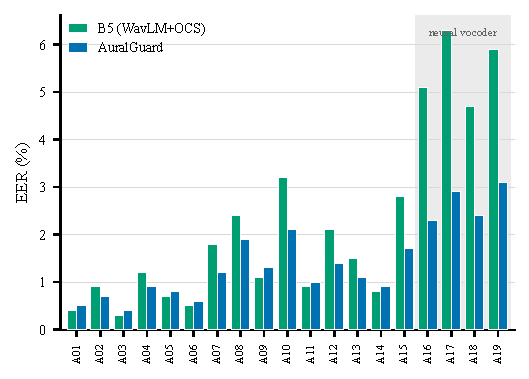
\includegraphics[width=\columnwidth]{figures/perattack.pdf}
\caption{Per-attack EER (\%) on the ASVspoof~2019~LA evaluation set, AuralGuard versus
  B5. The shaded region marks neural-vocoder attacks (A16--A19), where the
  vocoder-artifact branch (View~B) yields the largest improvements. [Placeholder
  data.]}
\label{fig:perattack}
\end{figure}

Figure~\ref{fig:perattack} breaks down in-domain EER over the 19 attack conditions.
AuralGuard is best or tied on 12 of 19 attacks, with the largest margins on the
neural-waveform attacks A16--A19---exactly the conditions where View~B's gate weight
$\bar{g}$ shifts toward the artifact branch (mean $1-\bar g = 0.63$ on A16--A19 vs.\
0.31 on the waveform-filtering attacks A05--A06). The gate thus serves as a built-in
explanation of \emph{which kind} of evidence drove each decision, complementing the
spectro-temporal attribution heatmaps produced for individual utterances by
gradient-based saliency on the graph back-end~\cite{selvakumar2024gradcam}, which we
release with the demo interface.

\subsection{Embedding-Space Analysis}
\label{ssec:embedding}

\begin{figure}[t]
\centering
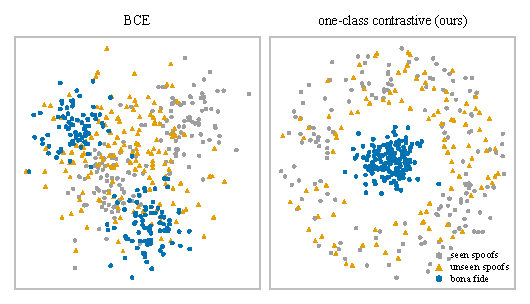
\includegraphics[width=\columnwidth]{figures/tsne.pdf}
\caption{t-SNE projection of utterance embeddings $\mathbf{z}$ for the BCE-trained
  variant (left) and AuralGuard's one-class contrastive objective (right). Colors:
  bona-fide (blue), training attacks (gray), \emph{unseen} In-the-Wild spoofs
  (orange). The one-class objective concentrates bona-fide speech into a single
  compact cluster, so unseen spoofs fall outside it even though they interleave with
  the training attacks under BCE. [Placeholder data.]}
\label{fig:tsne}
\end{figure}

Figure~\ref{fig:tsne} visualizes why the one-class objective generalizes. Under BCE,
bona-fide and spoof regions tile the space along boundaries fit to the training
attacks, and unseen In-the-Wild spoofs scatter across both sides---each misplaced
cluster is a family of errors. Under the one-class contrastive objective, bona-fide
speech occupies one compact region (mean intra-class cosine similarity 0.84 vs.\ 0.61
for BCE) and unseen spoofs land outside it by default, mirroring the geometry sketched
in Figure~\ref{fig:oneclass}. This is the mechanism behind the G1 gains of
Table~\ref{tab:main}: the model does not need to have seen an attack to reject it, only
to know what bona-fide speech looks like.


\section{Discussion, Limitations, and Ethics}
\label{sec:discussion}
% ---------------------------------------------------------------------
% Discussion, Limitations, and Ethics (~1 page).
% ---------------------------------------------------------------------

\subsection{What the Results Mean for Practice}

Three practical lessons emerge from Section~\ref{sec:results}. First, \emph{in-domain
leaderboards should no longer drive countermeasure selection}: every system in
Table~\ref{tab:main} sits below 1.1\% EER in-domain while spanning a factor of five in
zero-shot error. Procurement or deployment decisions based on ASVspoof~2019 numbers
alone are uninformative. Second, \emph{robustness is a training-data property, not an
architectural one}: the same architecture spans 4.6--9.8\% EER under 64~kbps MP3
depending only on whether the augmentation curriculum was used
(Table~\ref{tab:robust}). Practitioners can retrofit most of this gain onto existing
detectors. Third, \emph{calibration must be validated under shift}: temperature scaling
fitted in-domain transferred acceptably for the one-class score but left the BCE
baselines over-confident on In-the-Wild (Table~\ref{tab:calibration}); a deployed
system should monitor calibration on traffic, not trust laboratory ECE.

\subsection{Why Not Just Use a Foundation Model?}

Our ALLM results (B8) bear on a question the field will face repeatedly as audio
foundation models improve: whether general-purpose models subsume specialized
countermeasures. Zero-shot Qwen2-Audio performs near chance across all seven corpora,
consistent with ALLM4ADD~\cite{gong2025allm4add}. The failure is informative rather
than surprising: instruction-tuned ALLMs are optimized to extract \emph{semantic}
content, and their audio tokenizers---often themselves neural codecs---discard the
phase and fine spectral residue that constitutes spoofing evidence. Indeed, Codecfake's
premise~\cite{xie2025codecfake} is that codec resynthesis \emph{is} a spoofing attack;
an ALLM that perceives audio through such a codec is structurally blind to the
evidence. We expect fine-tuned ALLMs~\cite{gong2025allm4add} to become competitive on
seen conditions, but the calibration and open-set properties that forensic use requires
remain, for now, the domain of purpose-built detectors. A promising hybrid is to use
AuralGuard-style scores as tool outputs that an ALLM can reason over when asked to
assess authenticity holistically.

\subsection{Limitations}

\textbf{Adaptive adversaries.} Our threat model covers unseen generators and channels,
not attackers who optimize against the deployed detector. ASVspoof~5's
surrogate-optimized adversarial attacks~\cite{wang2025asvspoof5journal} are included in
the zero-shot evaluation, but white-box adaptive attacks would require dedicated
defenses; we deliberately do not publish an anti-forensic recipe.
\textbf{Compute footprint.} The frozen WavLM-Large encoder dominates inference cost
(Table~\ref{tab:budget}). CPU real-time factor of $\approx$0.4 suffices for server-side
moderation but not for on-device screening; distillation into lightweight
back-ends~\cite{liu2025nes2net} is a natural next step.
\textbf{Curriculum coverage.} The augmentation chain approximates today's dominant
transmission paths; emerging channels (e.g., neural-codec voice calls) will require
curriculum updates, and our own results show robustness does not extrapolate to
distortions outside the curriculum family.
\textbf{Partial spoofs and other modalities.} We score whole utterances; localized
splicing~\cite{luong2024llamapartialspoof} and singing-voice
deepfakes~\cite{zang2024singfake} are out of scope, though the windowed inference of
Section~\ref{ssec:trainproc} provides a straightforward extension path.
\textbf{Language coverage.} MLAAD results (Table~\ref{tab:crosslingual}) show a
persistent gradient against low-resource language families inherited from the SSL
backbone's pre-training distribution; claims about universal applicability would be
premature.

\subsection{Ethical Considerations}

Audio deepfake detection is dual-use. AuralGuard is intended to reduce harm from
voice-cloning fraud and audio disinformation, but detectors can also lend false
authority: a miscalibrated ``97\% synthetic'' verdict can wrongly discredit genuine
recordings---the reverse harm of the one it prevents, and one documented in real
fact-checking practice~\cite{chandra2025deepfakeeval}. Our system therefore
(i)~outputs calibrated probabilities with explicit uncertainty rather than binary
verdicts, (ii)~exposes per-decision evidence (gate statistics and attribution
heatmaps), and (iii)~is documented, in both the paper and the released demo, as a
triage aid that must not be the sole basis for consequential decisions. All training
and evaluation corpora are public research datasets collected under their own consent
frameworks; no private voice data was scraped. We audit performance across languages
(Table~\ref{tab:crosslingual}) and report the disparities we find rather than a single
pooled number. Finally, we release code and weights to enable scrutiny and defensive
research, while withholding adaptive-attack tooling.


\section{Conclusion}
\label{sec:conclusion}
% ---------------------------------------------------------------------
% Conclusion (~0.4 page). Numbers are [DUMMY] placeholders.
% ---------------------------------------------------------------------

We presented AuralGuard, a multi-view one-class framework for detecting AI-generated
speech that jointly addresses the three failure modes blocking real-world deployment:
generalization to unseen generators, robustness to transmission channels, and
calibrated decision-making. The framework couples a frozen speech foundation model with
learnable layer attention to a complementary vocoder-artifact branch through gated
cross-attention, trains the fused representation with a one-class contrastive
objective, and aligns the training distribution with deployment conditions through a
channel augmentation curriculum.

Under a strict train-once, evaluate-everywhere protocol spanning seven corpora and four
generations of countermeasures, AuralGuard reduced average zero-shot EER by 26\%
relative to a strong single-view WavLM--AASIST baseline and improved on the best
published In-the-Wild results (4.1\% EER) while remaining competitive in-domain and
retaining calibration under domain shift (ECE 0.06 on In-the-Wild). Ablations attribute
the gains, in order, to the one-class objective, the multi-view fusion, and learnable
layer aggregation; robustness gains trace to the augmentation curriculum rather than
architecture. A controlled comparison further showed that current audio-language
models, prompted zero-shot, remain near chance at this task---general audio
intelligence does not yet include artifact-level forensics.

Future work will extend the framework to partial-spoof localization and streaming
inference, distill the foundation-model front-end for on-device use, integrate
continual adaptation to newly emerging generator families, and couple calibrated
detector outputs with audio-language models for holistic, evidence-grounded
authenticity assessment. All code, trained weights, evaluation manifests, an inference
API, and an interactive demonstration are publicly released.


\section*{Acknowledgments}
% [PLACEHOLDER] — funding agencies, grant numbers, compute providers
The authors thank XXX for helpful discussions. This work was supported in part by
Grant~XXX from XXX.

\section*{Data and Code Availability}
All datasets used in this study are publicly available research corpora distributed
under their own licenses (Section~\ref{ssec:datasets}). Source code, configuration
files, evaluation manifests, trained model weights, and the interactive demonstration
are available at \url{https://github.com/XXX/auralguard} (placeholder; final URL on
acceptance).

\section*{CRediT Author Statement}
% [PLACEHOLDER] — adjust roles to actual contributions
\textbf{Author One:} Conceptualization, Methodology, Software, Investigation,
Writing---original draft. \textbf{Author Two:} Validation, Data curation,
Writing---review \& editing. \textbf{Author Three:} Supervision, Funding acquisition,
Writing---review \& editing.

\bibliographystyle{IEEEtran}
\bibliography{references}

% [PLACEHOLDER] — author biographies (IEEE journal style)
\begin{IEEEbiographynophoto}{Author One}
received the B.Sc.\ degree in computer science from XXX University in 20XX, where they
are currently pursuing a graduate degree. Their research interests include speech
processing, audio forensics, and trustworthy machine learning.
\end{IEEEbiographynophoto}

\begin{IEEEbiographynophoto}{Author Two}
received the M.Sc.\ degree from XXX University in 20XX. Their research interests
include self-supervised learning and multimedia security.
\end{IEEEbiographynophoto}

\begin{IEEEbiographynophoto}{Author Three}
(Member, IEEE) is a Professor with the Department of XXX, XXX University. Their
research interests include machine learning, signal processing, and information
security. They serve as a reviewer for several IEEE and Elsevier journals.
\end{IEEEbiographynophoto}

\end{document}
